%% Bayesian Networks Research

\documentclass[11pt,a4paper]{report}

%%------------------------------- preamble ------------------------------------

%% comment next for EN
\usepackage[utf8]{inputenc}       % accents
\usepackage[T1]{fontenc}          % PS fonts
\usepackage{newtxtext,newtxmath}  % do not use CM fonts
\usepackage{amsmath}              % multi-line and other mathematical statements
\usepackage{setspace}             % setting the spacing between lines
\usepackage{graphicx}             % go far beyond what the graphics package
\usepackage[normalem]{ulem}       % various types of underlining
\usepackage{caption}              % rotating captions, sideways captions, etc.
\usepackage{float}                % tables and figures in the multi-column environment 
\usepackage{subcaption}           % for subfigures and the like
\usepackage{longtable}            % tables that continue to the next page
\usepackage{multirow}             % tabular cells spanning multiple rows
\usepackage[table]{xcolor}        % driver-independent color extensions
\usepackage{lipsum}               % loren dummy text
\setlength{\marginparwidth}{2cm}  % todonotes' requirements
\usepackage{todonotes}            % todo's
\usepackage{chicago}              % a bibliography style
\usepackage{tabularx}
\usepackage{graphicx}
%% document dimensions
\usepackage[a4paper,left=25mm,right=25mm,top=25mm,bottom=25mm,headheight=6mm,footskip=12mm]{geometry}
\setlength{\parindent}{0em}
\setlength{\parskip}{1ex}

%% headers & footers
\usepackage{lastpage}
\usepackage{fancyhdr}
\fancyhf{}                            % clear off all default fancyhdr headers and footers
\rhead{\small{\emph{\projtitle, \projauthor}}}
\rfoot{\small{\thepage\ / \pageref{LastPage}}}
\pagestyle{fancy}                     % apply the fancy header style
\renewcommand{\headrulewidth}{0.4pt}
\renewcommand{\footrulewidth}{0.4pt}

%% colors
\usepackage{color}
\definecolor{engineering}{rgb}{0.549,0.176,0.098}
\definecolor{cloudwhite}{cmyk}{0,0,0,0.025}

%% source-code listings
\usepackage{listings}
\lstset{ %
 language=Python,                        % choose the language of the code
 basicstyle=\footnotesize\ttfamily,
 keywordstyle=\bfseries,
 numbers=left,                      % where to put the line-numbers
 numberstyle=\scriptsize\texttt,    % the size of the fonts that are used for the line-numbers
 stepnumber=1,                      % the step between two line-numbers. If it's 1 each line will be numbered
 numbersep=8pt,                     % how far the line-numbers are from the code
 frame=tb,
 float=htb,
 aboveskip=8mm,
 belowskip=4mm,
 backgroundcolor=\color{cloudwhite},
 showspaces=false,                  % show spaces adding particular underscores
 showstringspaces=false,            % underline spaces within strings
 showtabs=false,                    % show tabs within strings adding particular underscores
 tabsize=2,                         % sets default tabsize to 2 spaces
 captionpos=b,                      % sets the caption-position to bottom
 breaklines=true,                   % sets automatic line breaking
 breakatwhitespace=false,           % sets if automatic breaks should only happen at whitespace
 escapeinside={\%*}{*)},            % if you want to add a comment within your code
 morekeywords={*,var,template,new}  % if you want to add more keywords to the set
}

%% hyperreferences (HREF, URL)
\usepackage{hyperref}
\hypersetup{
    plainpages=false, 
    pdfpagelayout=SinglePage,
    bookmarksopen=false,
    bookmarksnumbered=true,
    breaklinks=true,
    linktocpage,
    colorlinks=true,
    linkcolor=engineering,
    urlcolor=engineering,
    filecolor=engineering,
    citecolor=engineering,
    allcolors=engineering
}

%% path to the figures directory
\graphicspath{{figures/}}

%% macros, to be updated as needed
\newcommand{\school}{}
\newcommand{\degree}{}
\newcommand{\projtitle}{Bayesian Networks II: BN Inference}
\newcommand{\subtitle}{For Self-learning Purposes}
\newcommand{\projauthor}{Jiashu Chen}
\newcommand{\supervisor}{}
\newcommand{\tutor}{}

%% my other macros, if needed
\newcommand{\windspt}{\textsf{WindsPT\/}}
\newcommand{\windscannerpt}{\emph{Windscanner.PT\/}}
\newcommand{\class}[1]{{\normalfont\slshape #1\/}}
\newcommand{\svg}{\class{SVG}}
\newcommand{\mycomment}[1]{}

\graphicspath{ {./pics/} }

%% my environments for infos
\newenvironment{info}[1]{\vspace*{6mm}\color{blue}[ \textbf{INFO:} \begin{em} #1}
                        {\vspace*{3mm}\end{em} ]}
\newenvironment{infoopt}[1]{\vspace*{6mm}\color{blue}[ \textbf{INFO (elemento opcional):} \begin{em} #1}
                        {\vspace*{3mm}\end{em} ]}

%%------------------------------- document-------------------------------------

\begin{document}

%% preamble page numbers with roman numerals
\pagenumbering{roman}\setcounter{page}{1}
\pagestyle{plain}

%%------------------------------- cover page ----------------------------------

\begin{titlepage}
\center

\vspace{-15mm}
{\large \textbf{\textsc{\school}}}\\

\vfill

{\Large \textbf{\projtitle}}\\[8mm]
{\large \textbf{\subtitle}}\\[28mm]

{\Large \textbf{\projauthor}}\\

\vfill

%% includegraphics[width=52mm]{uporto-feup.pdf}

\vfill

%% {\large \degree}\\[8mm]
%\renewcommand{\today}{15 de dezembro de 2023}
\today

\end{titlepage}

%%------------------------------- table of contents ---------------------------

\tableofcontents

%%------------------------------- chapter ------------------------------------

\chapter{Recall: BN Representation}

%% display headers & footers
\pagestyle{fancy}
%% main page numbers with arabic numerals
\pagenumbering{arabic}\setcounter{page}{1}

\section{What is Bayesian Networks}

\begin{itemize}
    \item BN is a directed, acyclic graph, one node per random variable.
    \item A conditional probability table (CPT) for each node. A collection of distributions over X, one for each combination of parents'values.
    \begin{center}
        $P(X \mid a_{1}, \ldots, a_{n})$
    \end{center}
    \item Bayesian networks implicitely encode joint probability distributions.
    \begin{itemize}
        \item As a product of local conditional distributions
        \item To see what probability a BN gives to a full assignment, multiply all the relevant conditionals together.
        \begin{center}
            $P(x_{1}, x_{2}, \ldots, x_{n}) = \prod_{i=1}^{n}P(X_{1} \mid parents(X_{i}))$
        \end{center}
        \item If a node has no parent, then it is independent probability distribution. On the other hand, if nodes have many parents,  then the BN will become complicated. In general, we we want all variables connected but a small number of parents for each node so that each $P(X_{1} \mid parents(X_{i})$ term will be simple.
    \end{itemize}
    \item Example
    
    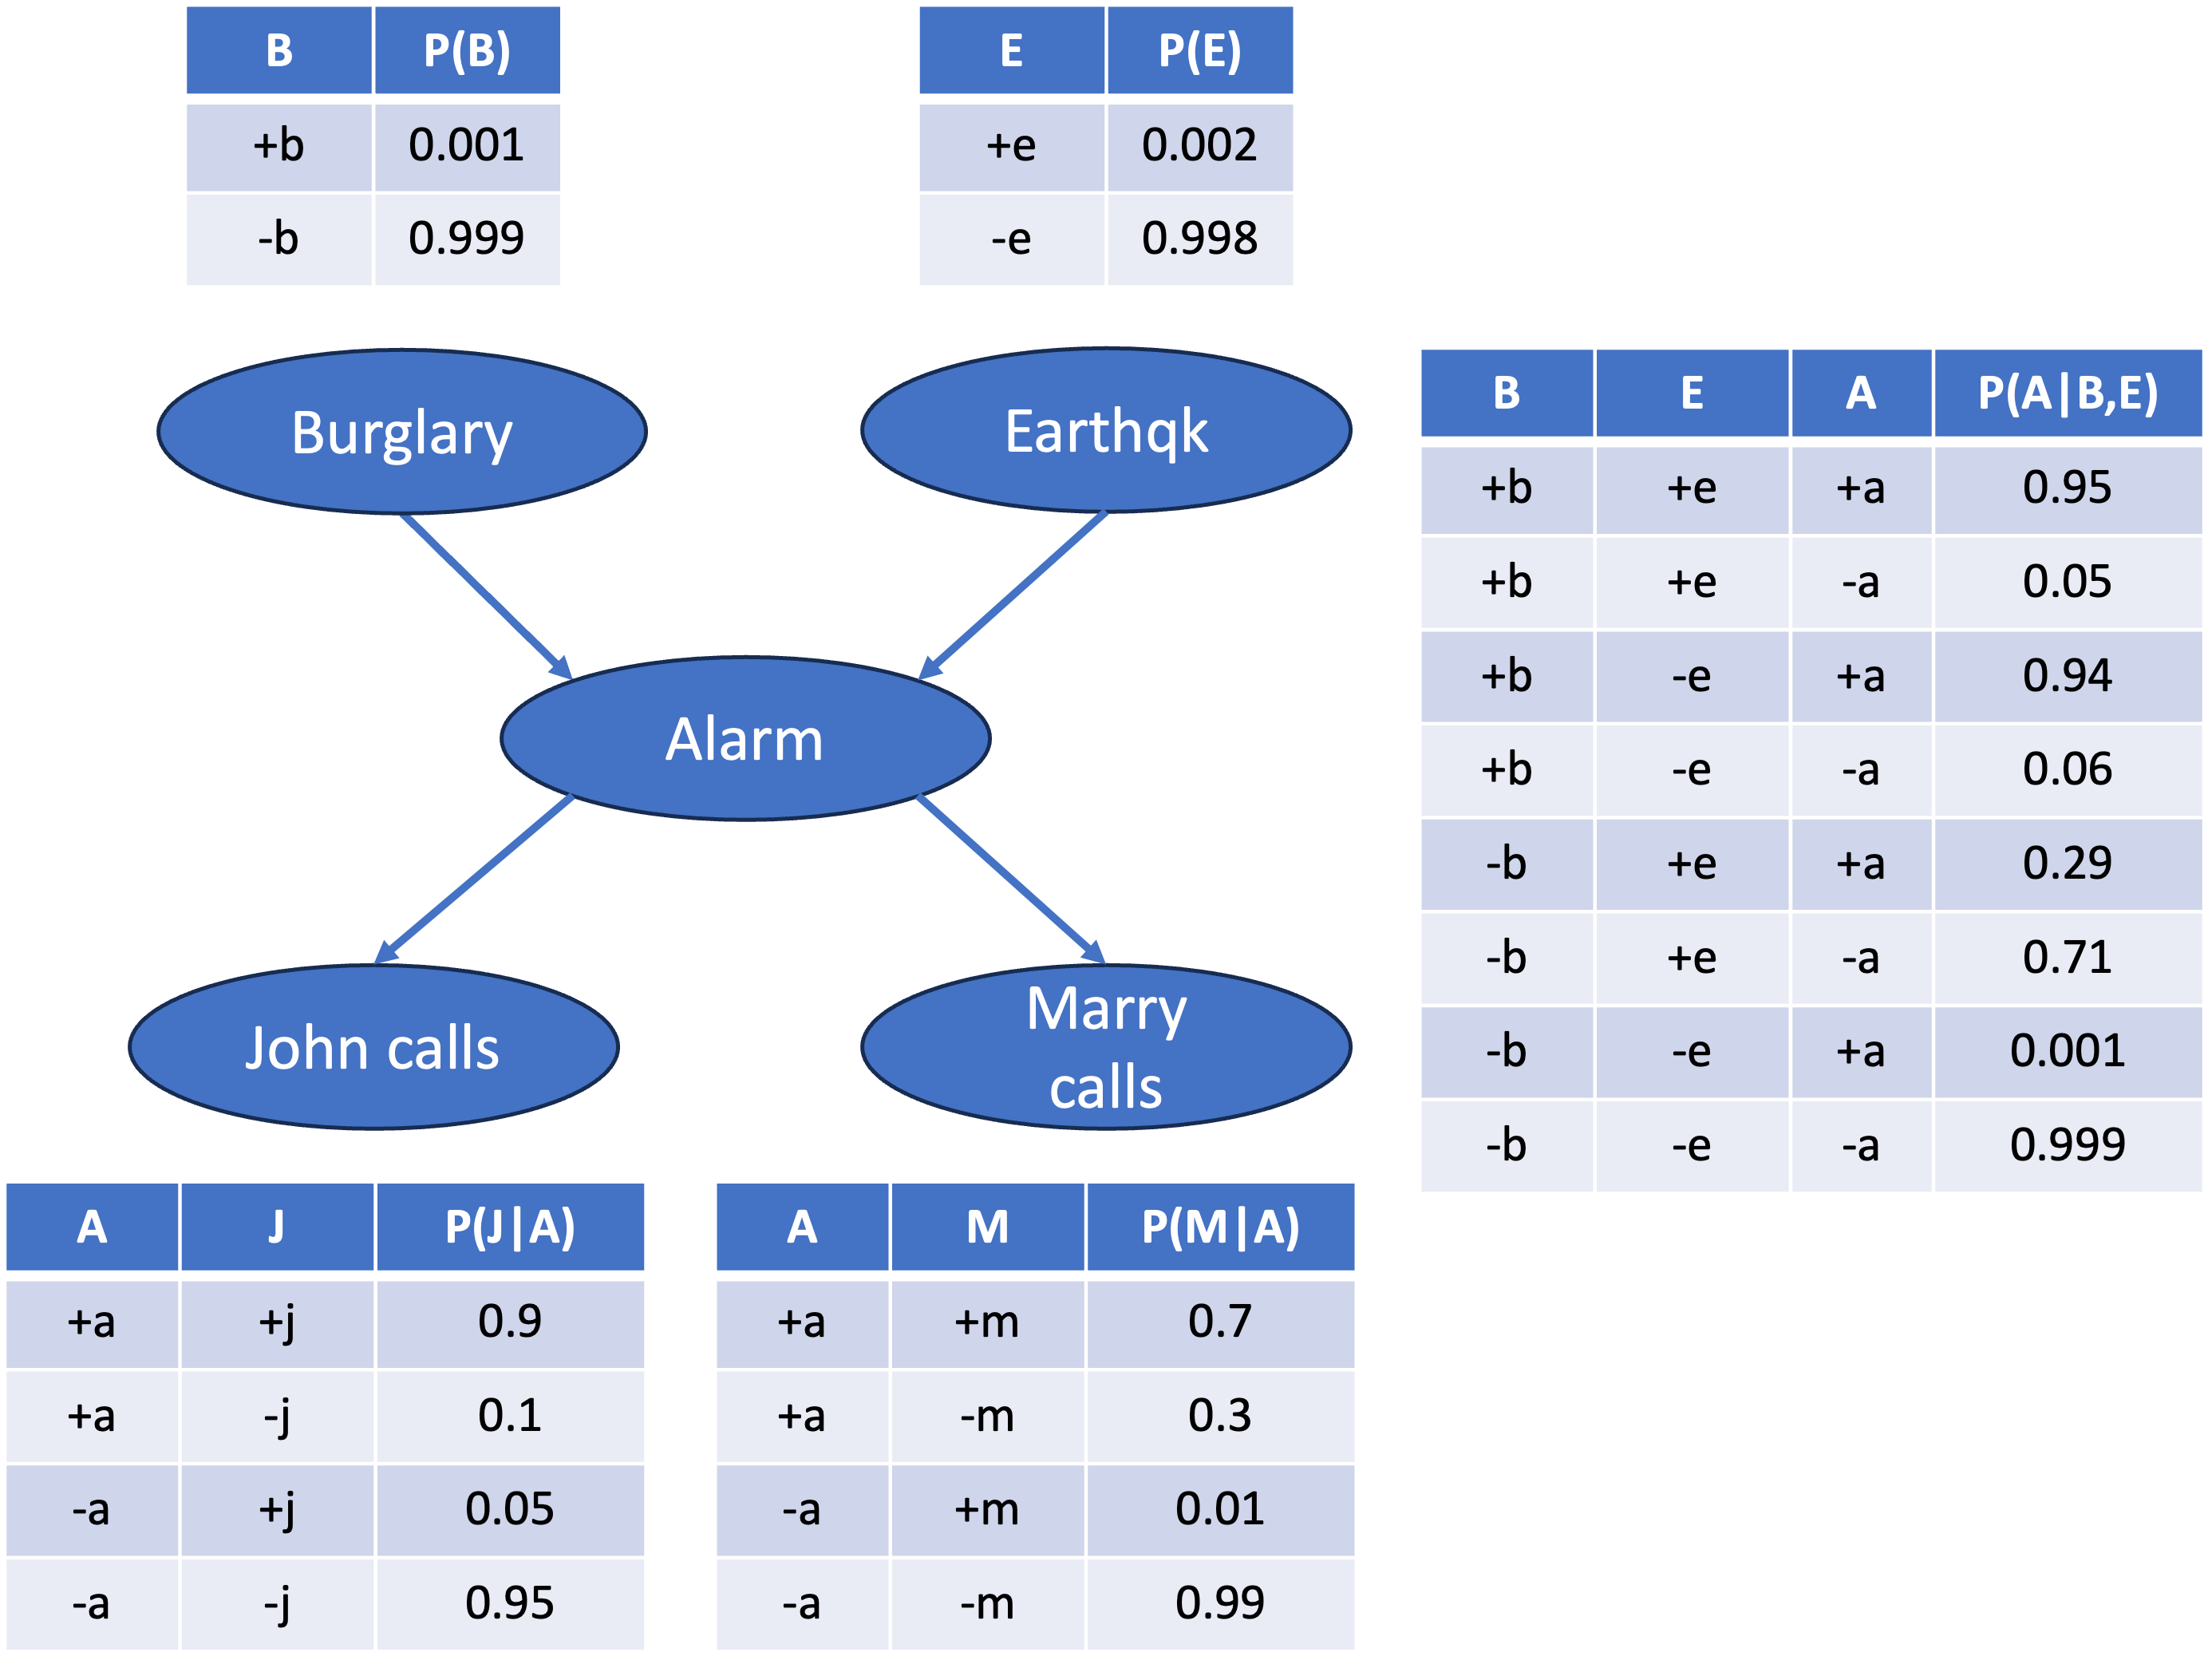
\includegraphics[width = 12cm, height=8cm]{alarm_eg.png}\\
    
    Suppose we want to compute the P(+b, -e, +a, -j, +m)
    \begin{center}
        $P(+b, -e, +a, -j, +m) = P(+b)P(-e)P(+a \mid +b, -e)P(-j \mid +a)P(+m \mid +a) = 0.001 * 0.998 * 0.94 * 0.1 * 0.7$
    \end{center}
\end{itemize}

%%------------------------------- chapter ------------------------------------

\chapter{Probabilistic Inference}

\section{Inference}

\begin{itemize}
    \item Inference: calculating some useful quantity from a joint probability distribution. For instance, posterior probaility $P(Q \mid E_{1} = e_{1}, \ldots, E_{k} = e_{k})$, most likely explanation $argmax_{q} P(Q = q \mid E_{1} = e_{1}, \ldots, E_{k} = e_{k})$
\end{itemize}

\section{Types of inferences}
    \begin{itemize}
        \item Causal Reasoning
        
        If there is a burglary, what is the probaility that John calls, P(j|b)?

        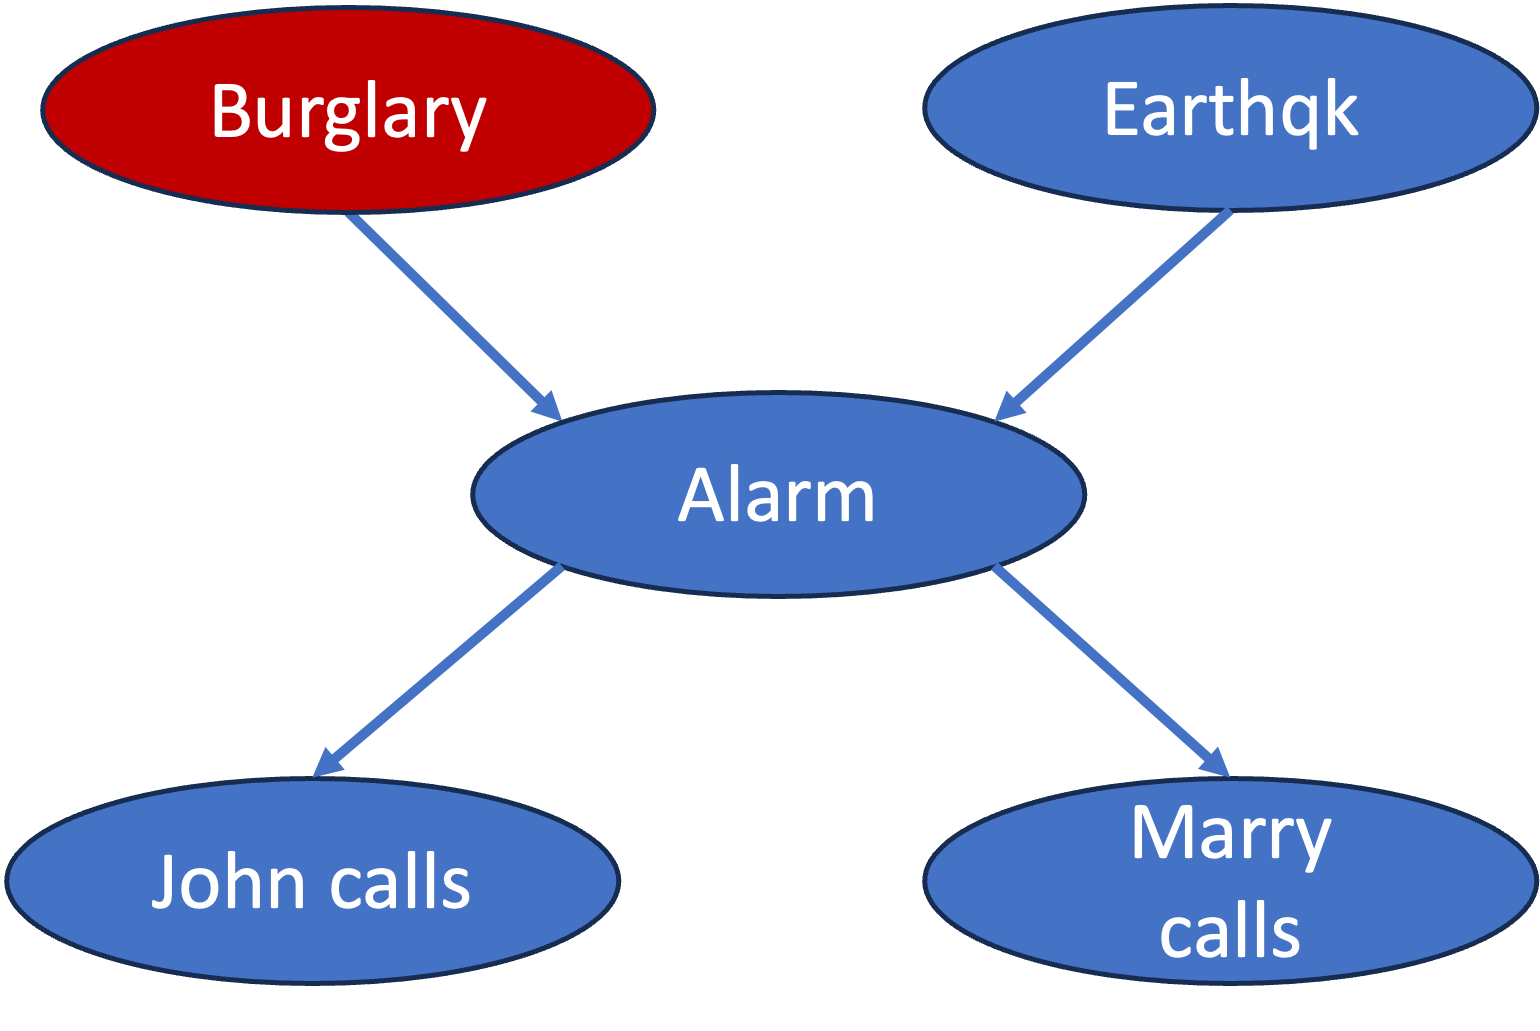
\includegraphics[width = 8cm, height = 5cm]{causal_reasoning.png}

        \item Evidential Reasoning
        
        If there is John calls, what is the probaility that there is a Burglary, P(b|j)?

        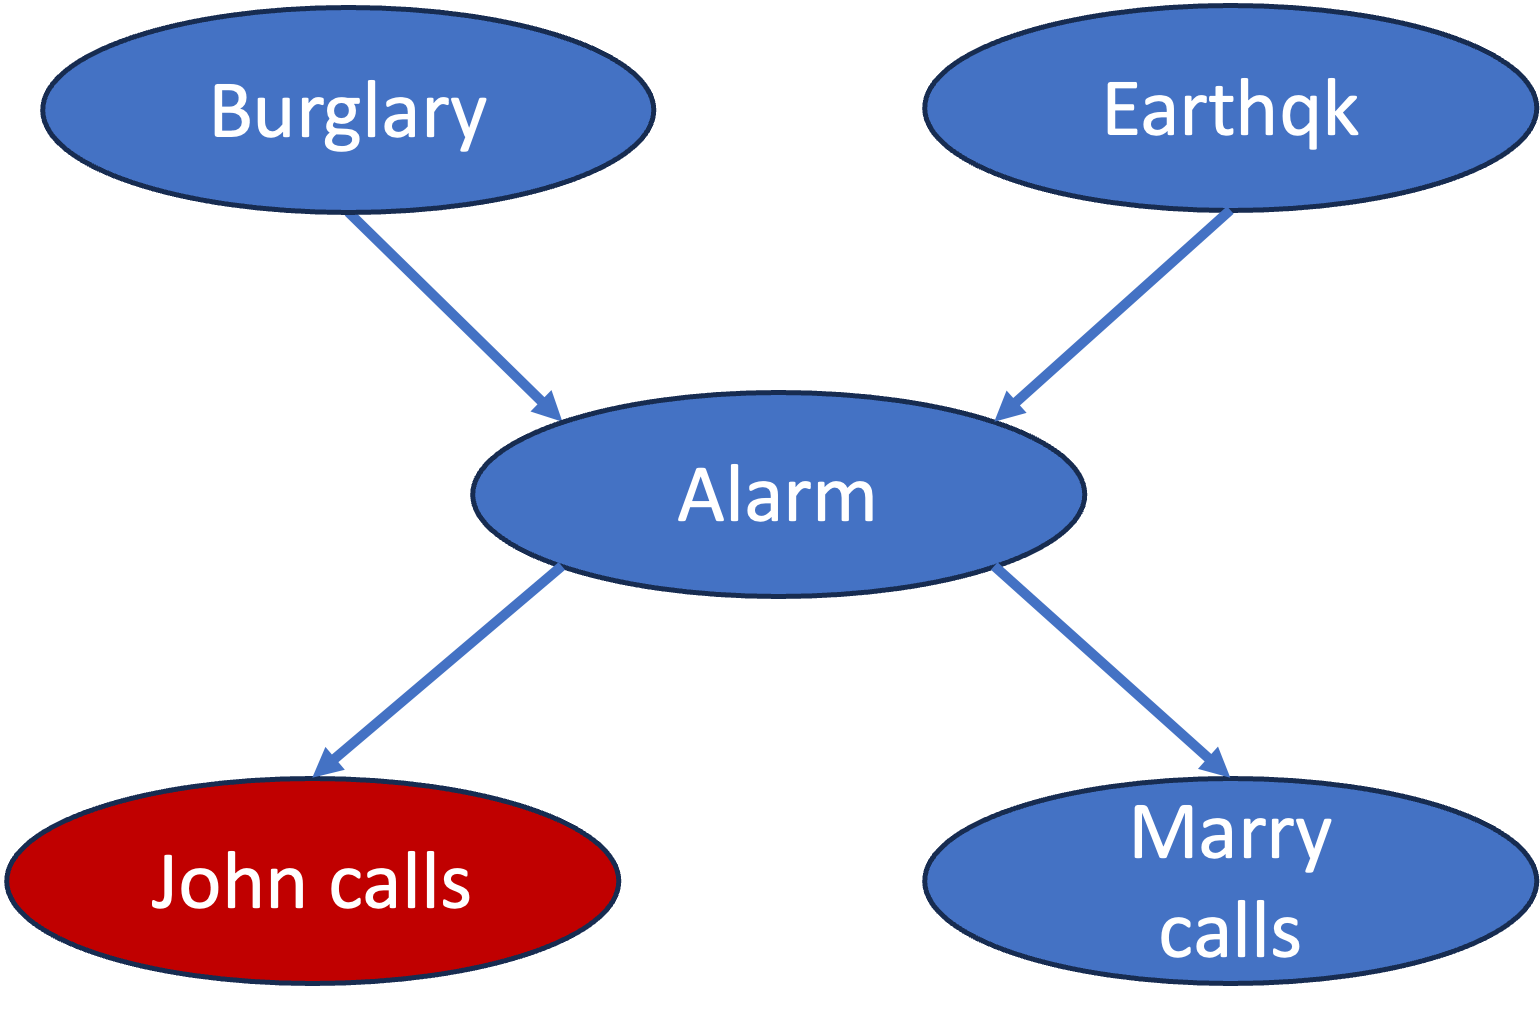
\includegraphics[width = 8cm, height = 5cm]{evidential_reasoning.png}

        \item Intercausal Reasoning
        
        If there is alarm, the probability of earthquake versus the probability of burglary P(b|a) versus P(e|a)?

        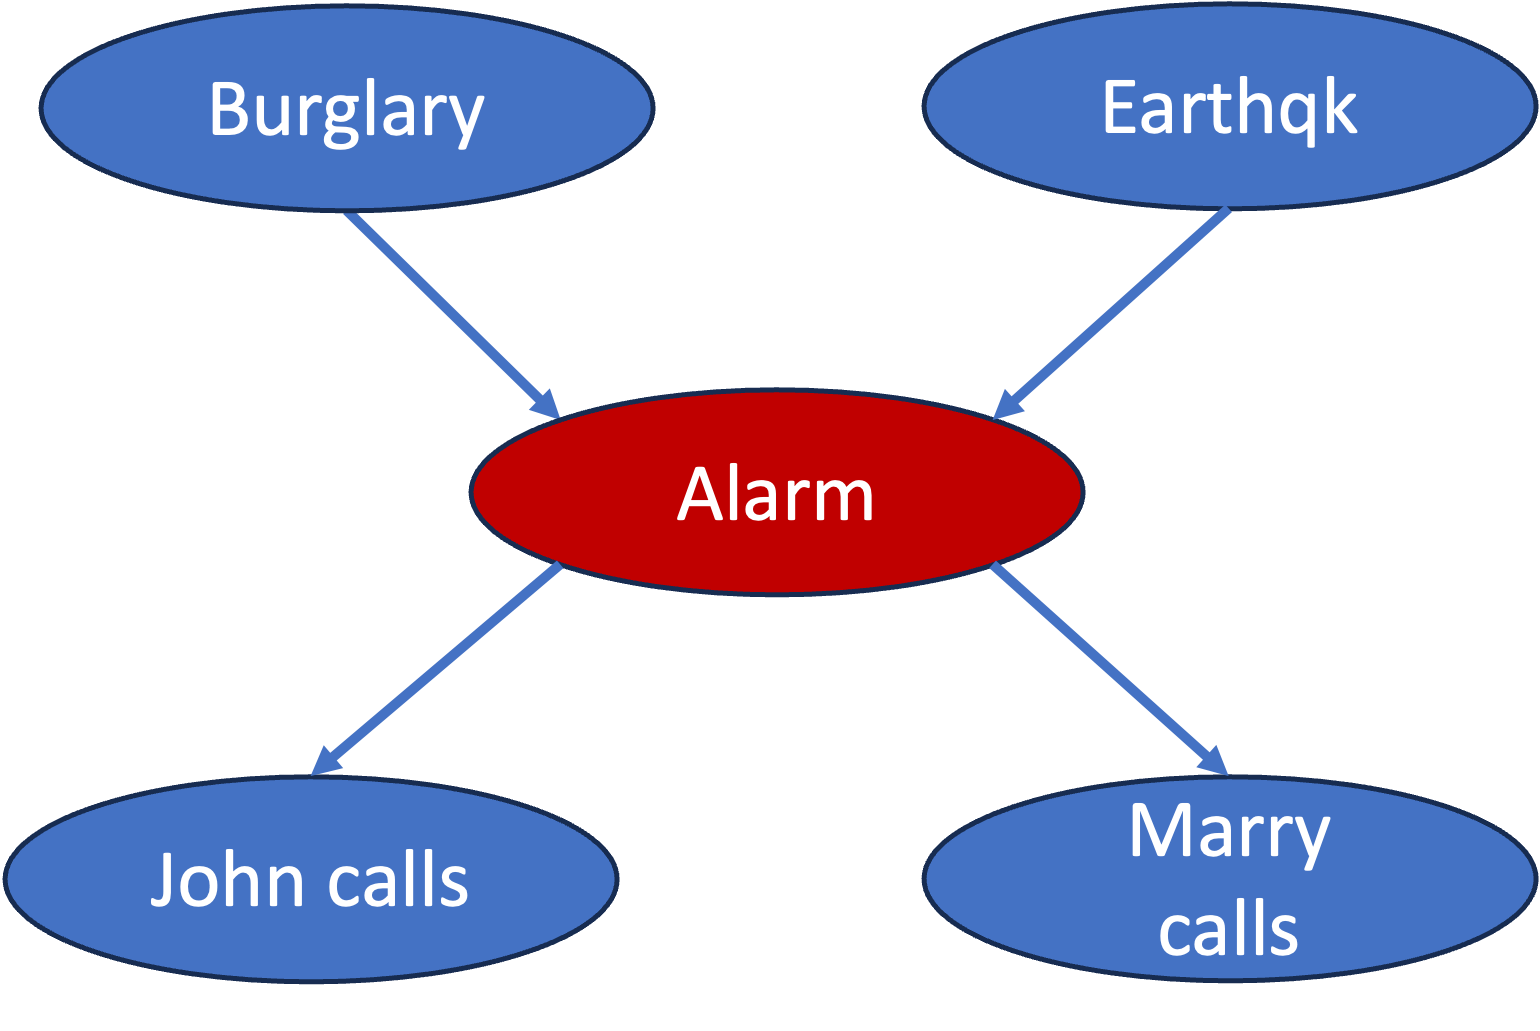
\includegraphics[width = 8cm, height = 5cm]{intercausal_reasoning.png}

        \item Intercausal Reasoning
        
        If there is alarm and burglary, what is the probability of earthquake? P(e|a,b)?

        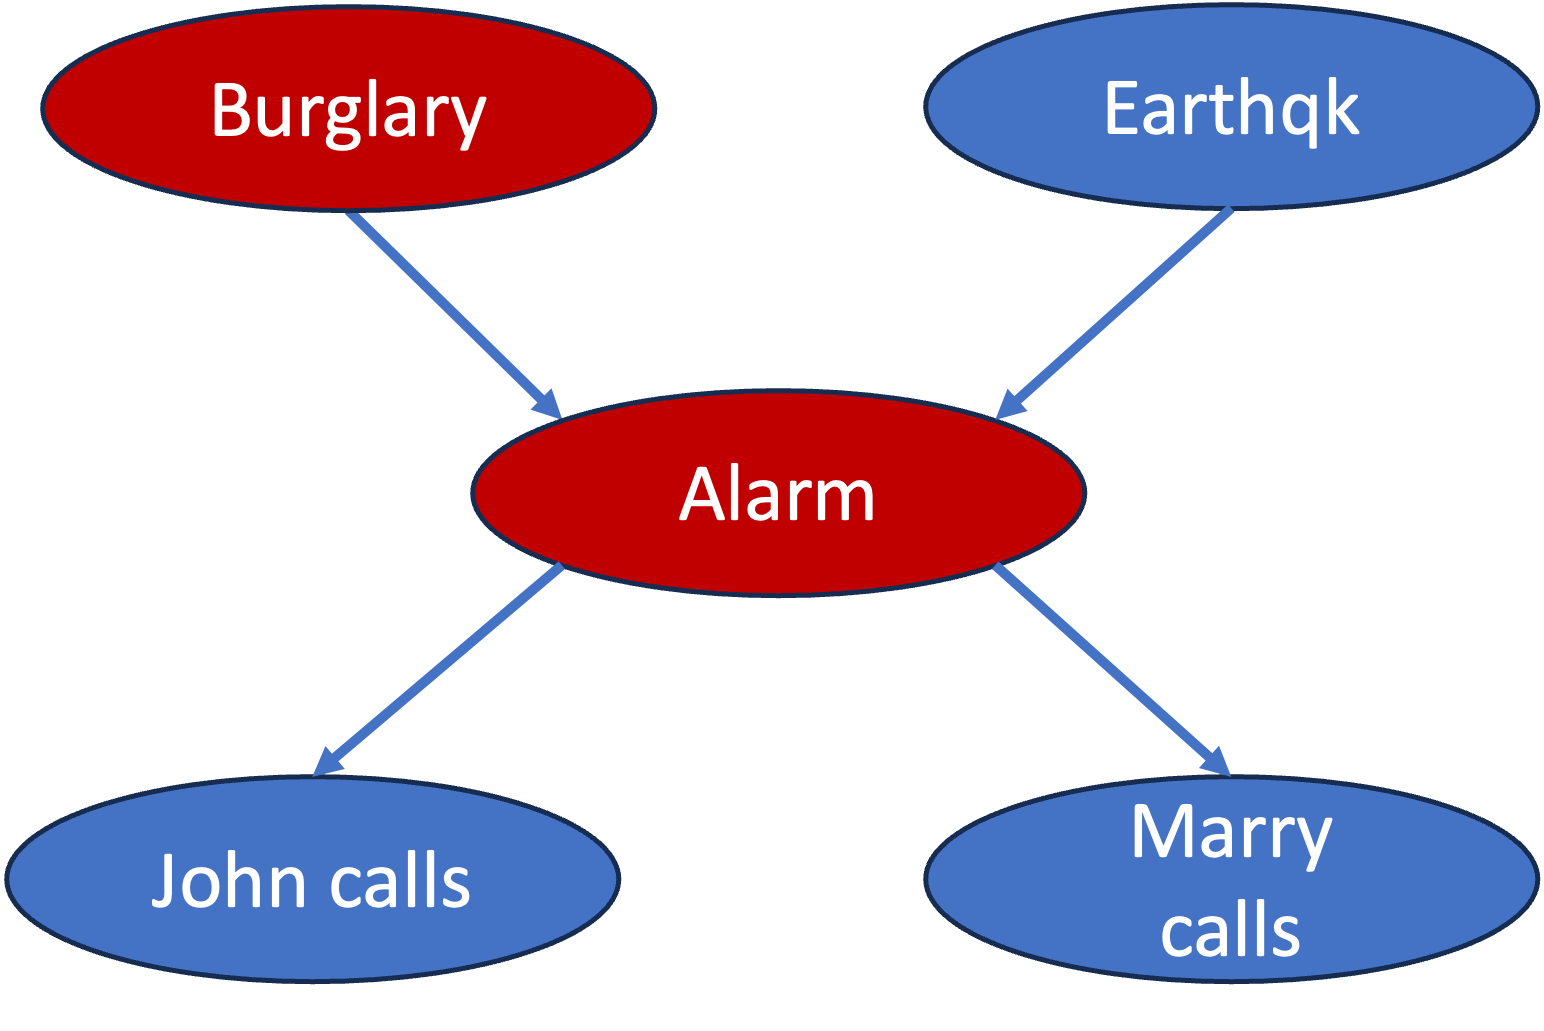
\includegraphics[width = 8cm, height = 5cm]{intercausal_reasoning2.png}

\end{itemize}

%%------------------------------- chapter ------------------------------------

\chapter{Inference by Enumeration}

\section{General Case}

All variables can be divided into three categories:

\begin{itemize}
    \item Evidential variables: $E_{1}, \ldots, E_{k} = e_{1}, \ldots, e_{k}$
    \item Query variable: Q
    \item Hidden variables: $H_{1}, \dots, H_{r}$
\end{itemize}

\section{Procedures}

\begin{itemize}
    \item Step1: select the entries consistent with evidence.
    \item Step2: Sum out H (marginalize hidden variables) to get joint probability of query and evidence. Results becomes one-dimmensional array where each row differs by the value of Q.
    \begin{center}
        $P(Q, e_{1}, \ldots, e_{k}) = \prod_{h_{1}, \ldots, h_{r}}P(Q, h_{1}, \ldots, h_{r}, e_{1}, \ldots, e_{k})$
    \end{center}
    \item Step3: Normalize
    \begin{center}
        $Z = \sum{q} P(Q, e_{1}, \ldots, e_{k})$

        $P(Q \mid e_{1}, \ldots, e_{k}) = \frac{1}{Z}P(Q, e_{1}, \ldots, e_{k})$
    \end{center}
\end{itemize}

\section{Problem with Enumeration}

\begin{itemize}
    \item Inference by enumeration is extremely slow (exponential time complexity), because we multiply all pieces of local conditional probabilities to form a exponential large joint probability. And then we collapse all variables we do not care about (hidden variables) to make it small again. We inflate and then deflate.
    \item Better idea: interleave joining and marginalizing (variable elimination).
\end{itemize}


%%------------------------------- chapter ------------------------------------

\chapter{Inference by Variable Elimination}


\section{Inference by Enumeration Versus Variable Elimination}

In enumeration, we join up the whole joint distribution before sum out hidden variables. In variable elimination, we join some variables and immediately sum out, and join next variables and sum out. We sum out hidden variables as soon as we can. Thus, we could control the growth speed. Variable elimination is still NP-hard, but it is ususally much faster than inference by enumeration.

\begin{itemize}
    \item Inference by Enumeration
    
    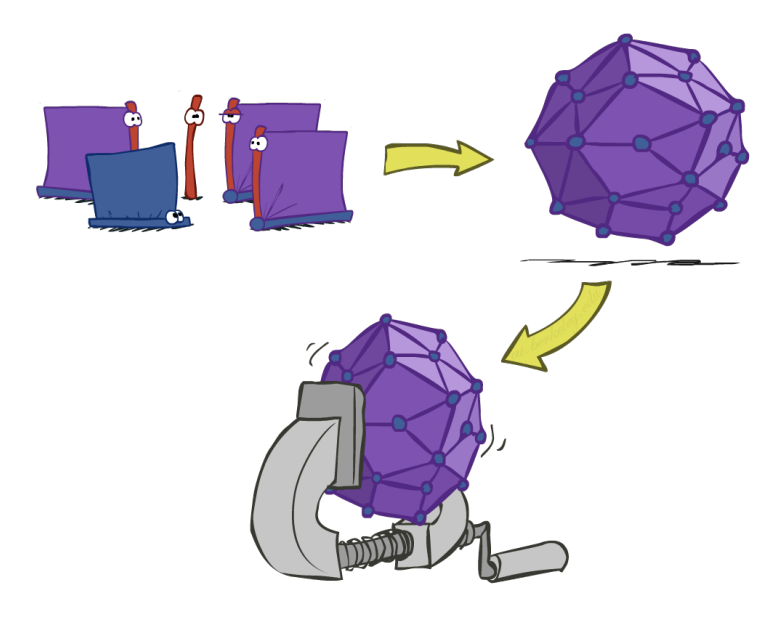
\includegraphics[width = 10cm, height = 5cm]{enumeration_slow.png}

    \item Variable Elimination
    
    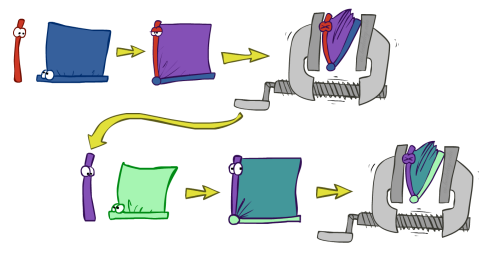
\includegraphics[width = 10cm, height = 5cm]{variable_elimination.png}

\end{itemize}

\section{Factors}

\begin{itemize}
    \item Joint distribution: P(X, Y)
        \begin{itemize}
            \item entries P(x, y) for all x, y
            \item sums to 1
            \item example: P(T, W) (2d array: the number of capital letters is the number of dimensionality.)
        \end{itemize}
    
    \item Selected join: P(x, Y)
        \begin{itemize}
            \item a slice of the joint distribution
            \item entries P(x, y) for fixed x, all y
            \item sums to P(x)
            \item example: P(cold, W) (1d array)
        \end{itemize}

    \item Single conditional: P(Y | x)
        \begin{itemize}
            \item entries P(y | x) for fixed x, all y
            \item sums to 1
            \item example: P(W, cold) (1d array)
        \end{itemize}

    \item Family of conditionals: P(Y | X)
        \begin{itemize}
            \item multiple conditionals
            \item entries P(y | x) for all x, y
            \item sums to |X|
            \item example: P(W | T) (2d array)
        \end{itemize}

    \item Specified family: P(y| X)
        \begin{itemize}
            \item entries P(y | x) for fixed y but for all x
            \item example: P(rain | T) (1d array)
        \end{itemize}
    
    \item Summary
        \begin{itemize}
            \item $P(Y_{1}, \ldots, Y_{n} \mid X_{1}, \ldots, X_{M})$
            \item It is a factor, a multi-dimensional array
            \item Its values are $P(y_{1}, \ldots, y_{n} \mid x_{1}, \ldots, x_{M})$
            \item Any assigned (lower case) X or Y is a dimension missing (or selected) from the array.
        \end{itemize}
    
\end{itemize}

\section{Traffic Example}

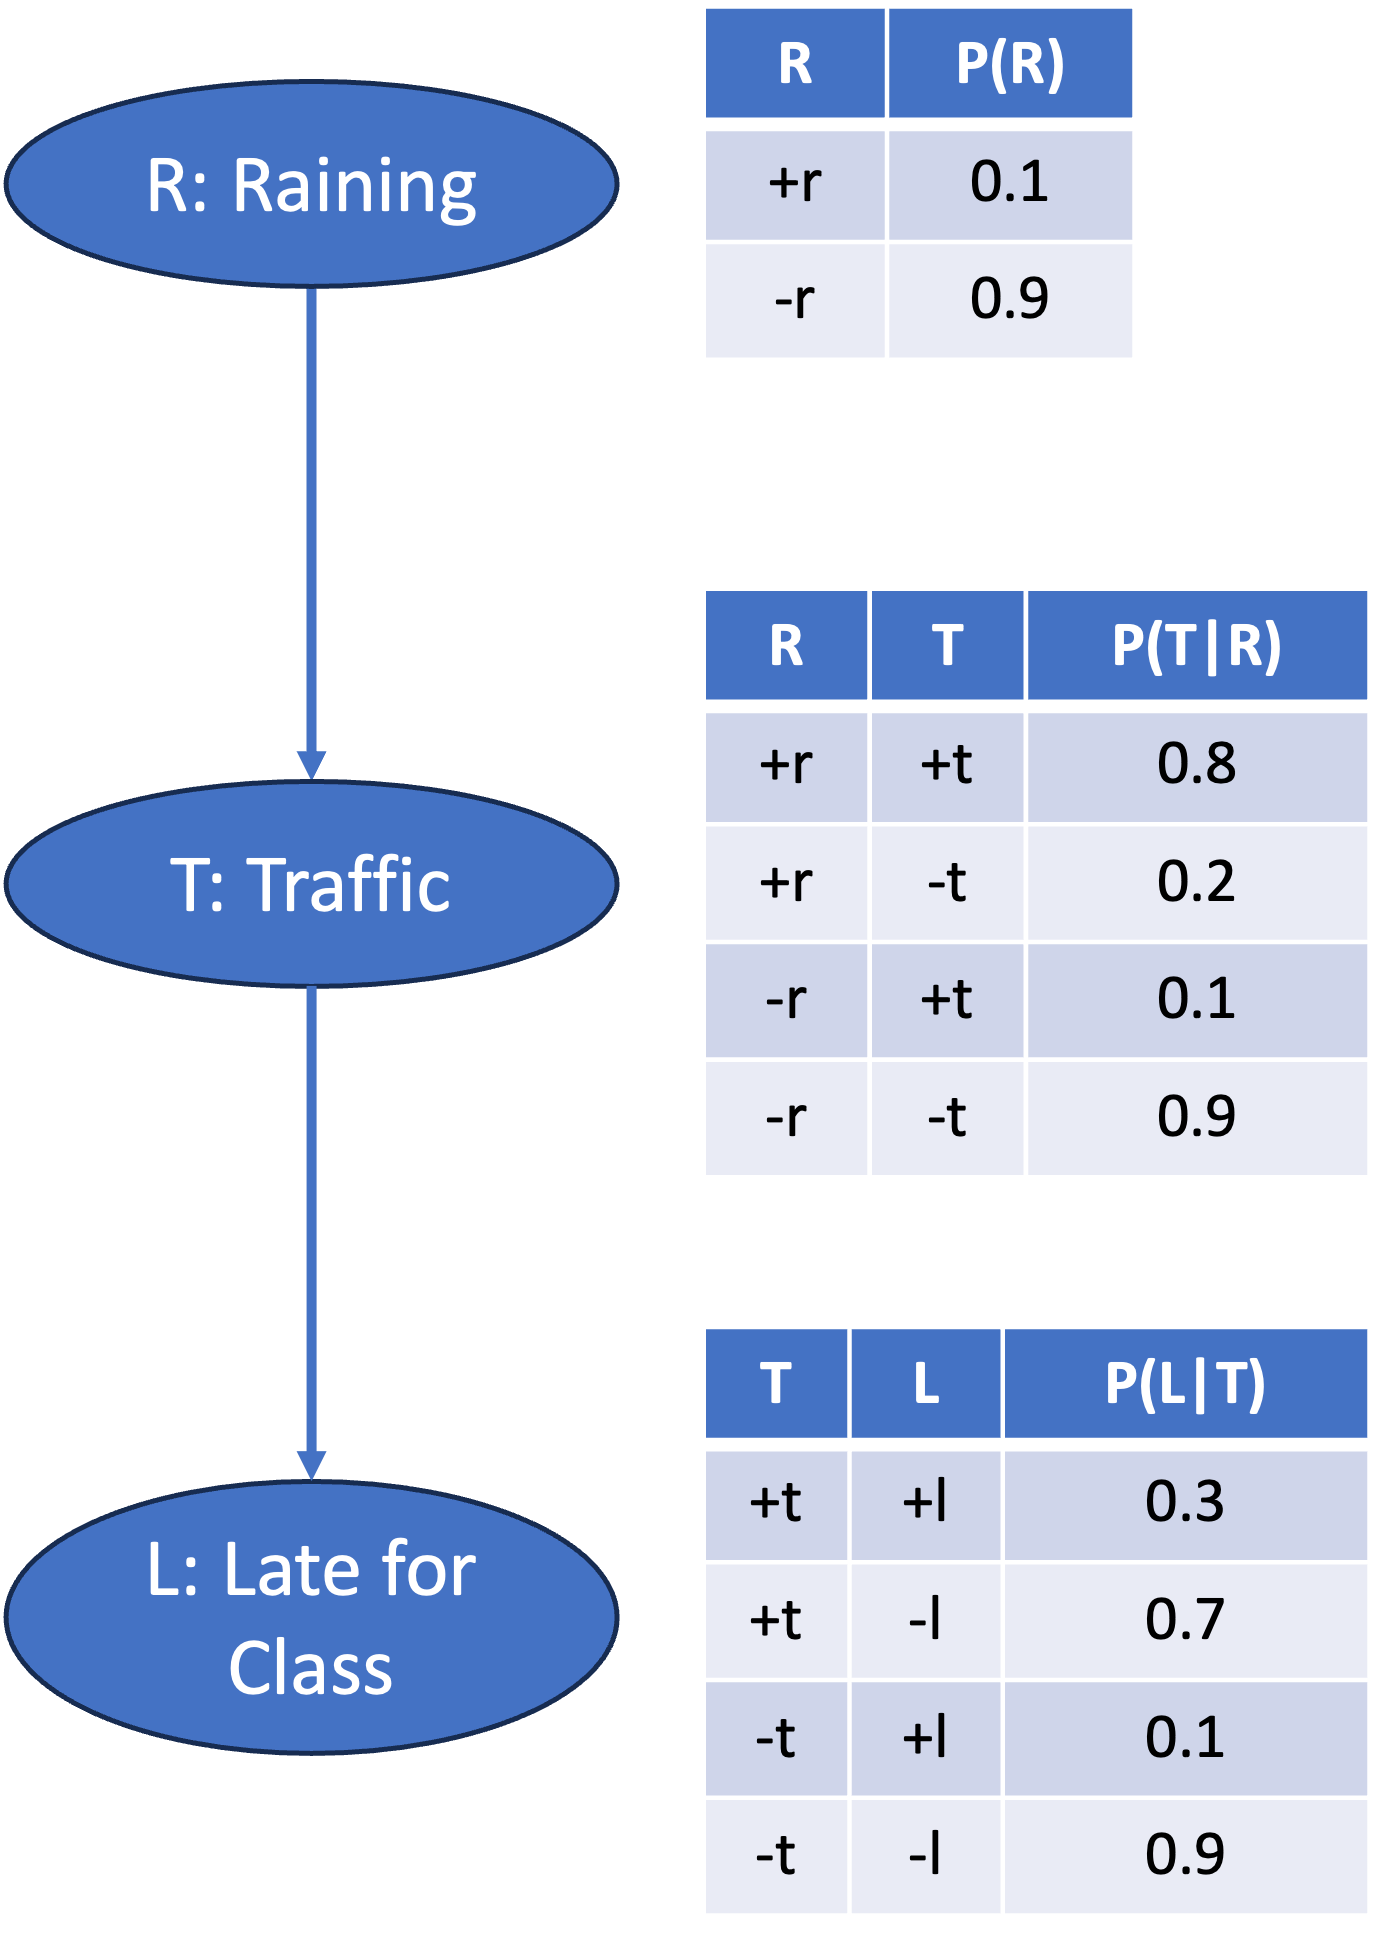
\includegraphics[width = 8cm, height = 10cm]{traffic_eg.png}

\begin{center}
    \begin{equation}
        \begin{split}
            P(L) & = ? \\
            & = \sum_{r,t}P(r,t,L) \\
            & = \sum_(r,t)P(r)P(t \mid r)P(L \mid t) \\
        \end{split}
    \end{equation}
\end{center}

\begin{itemize}
    \item Tracked objects called factors
    \item Initial factors are local CPTs (one per node)
    
    local CPTs are P(R), P(T|R), P(L|T)

    \item Any known values are selected

    suppose we know L = +l, the initial factors are P(R), P(T|R), P(+l|T)

    \item \textbf{Operation1: Join Factors (on X)}

        \begin{itemize}
            \item Combine factors just like a database join
            \item Get all factors over the joining variable (get all factors that include variable X)
            \item Build a new factor over the union of the variables involved.
            \item Example1: join on R
            
            It is like merging R and T into a mega variable (R, T)\\

            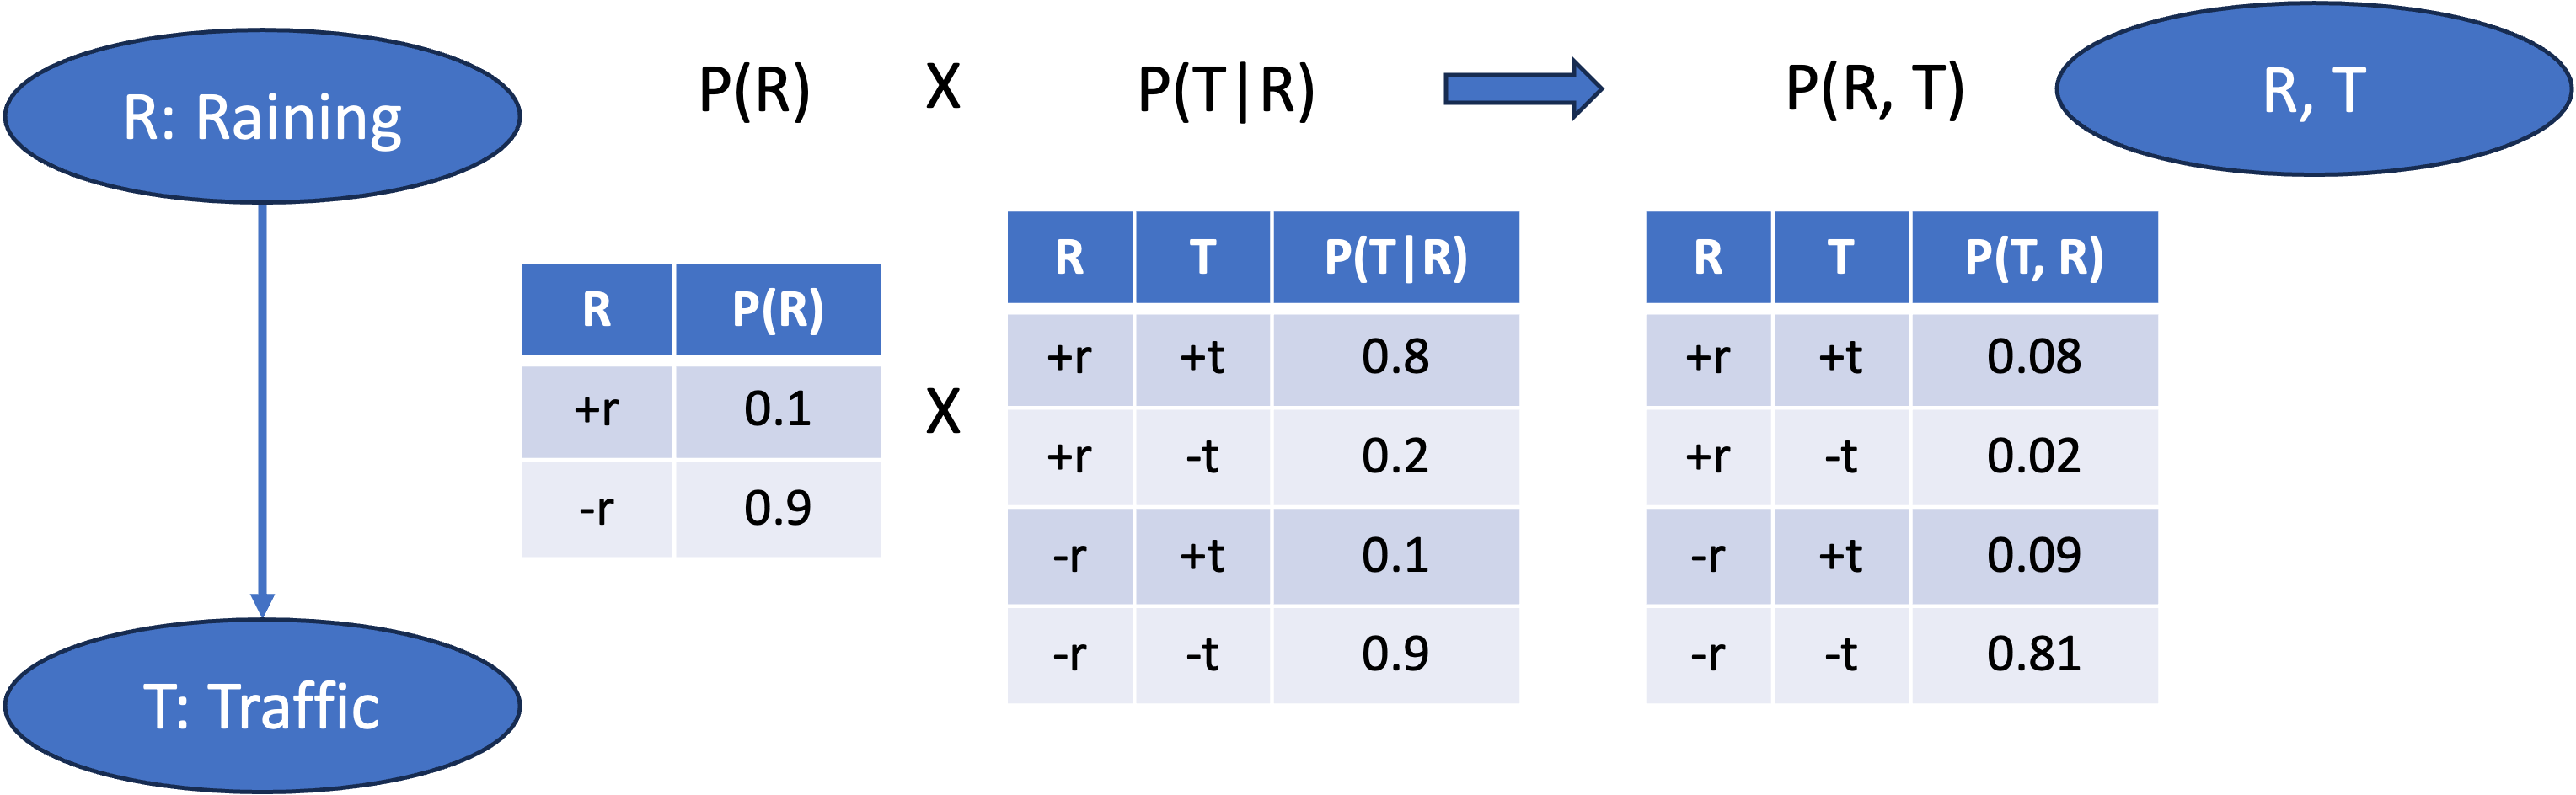
\includegraphics[width=15cm, height = 5cm]{op1_join.png}

            \item Example2: Multiple join
            
            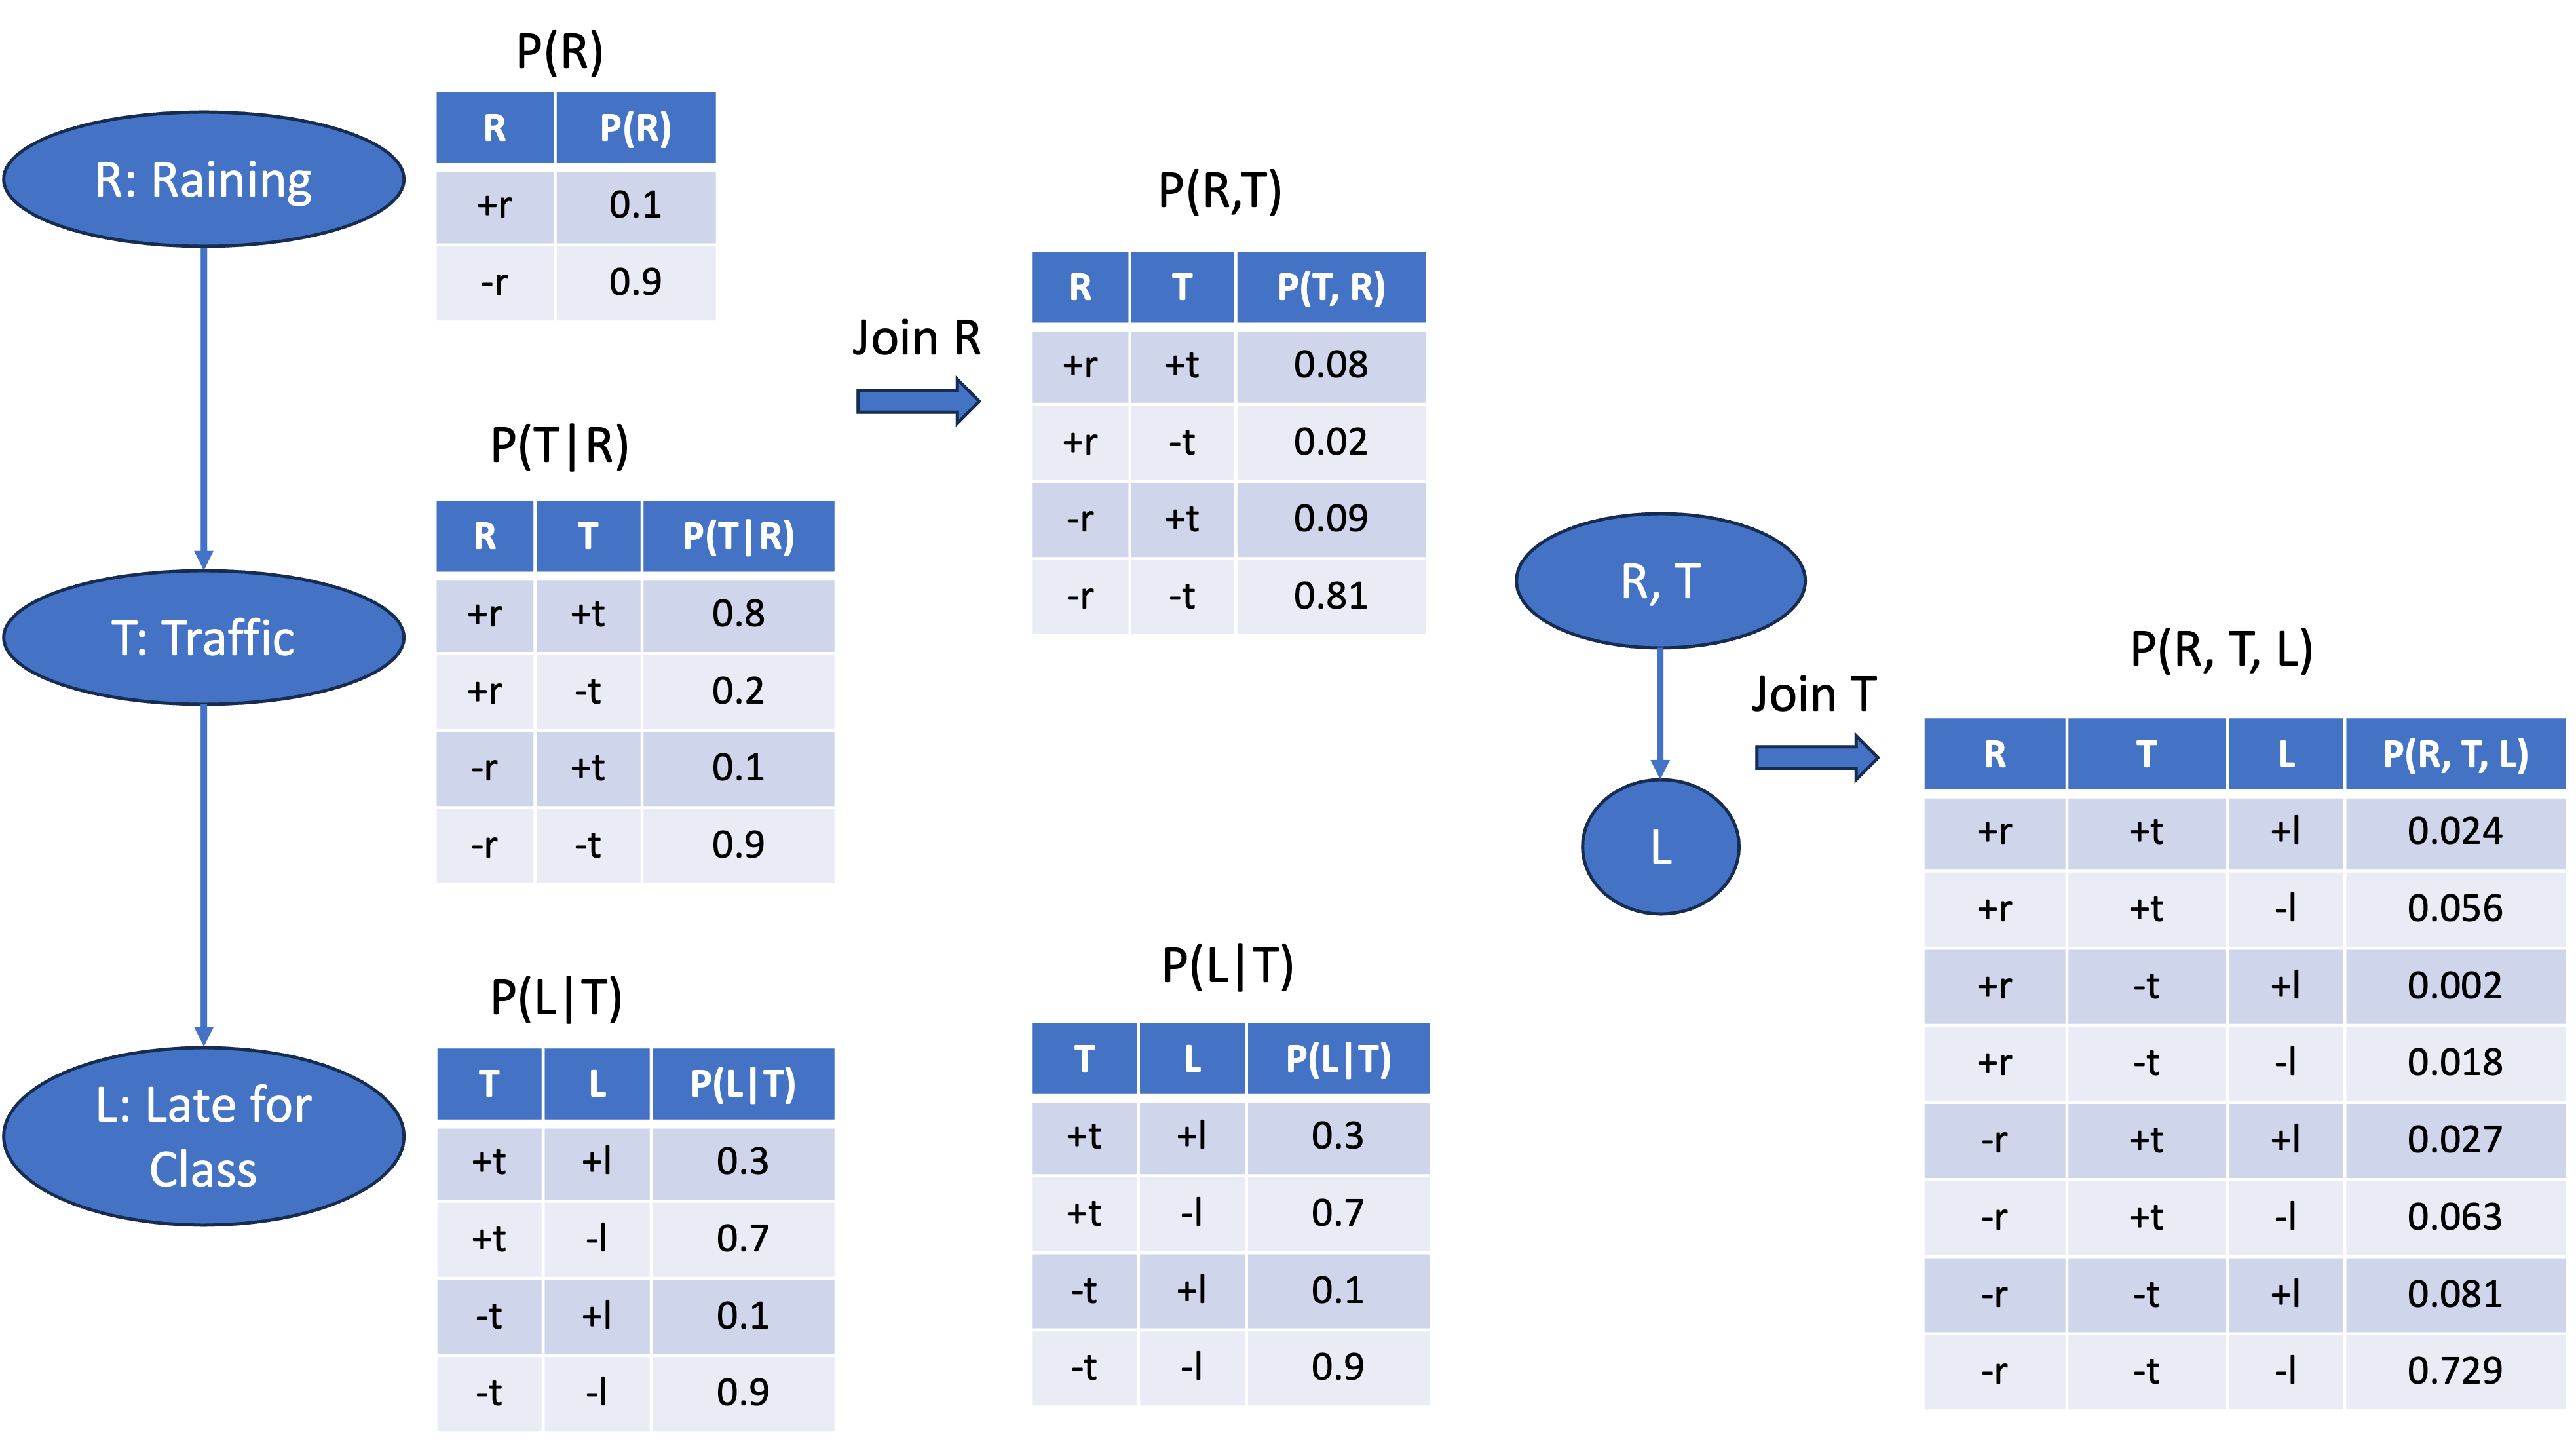
\includegraphics[width=16cm, height = 8cm]{op1_mul.png}
        \end{itemize}
    
    \item \textbf{Operation2: Elimination (Marginalization)}
        \begin{itemize}
            \item Take a factor and sum out a variable
            \item Shrinks a factor to a smaller one
            \item A projection operation
            \item Example1: Marginalization on R
            
            Collapsing 2d data to 1d\\
            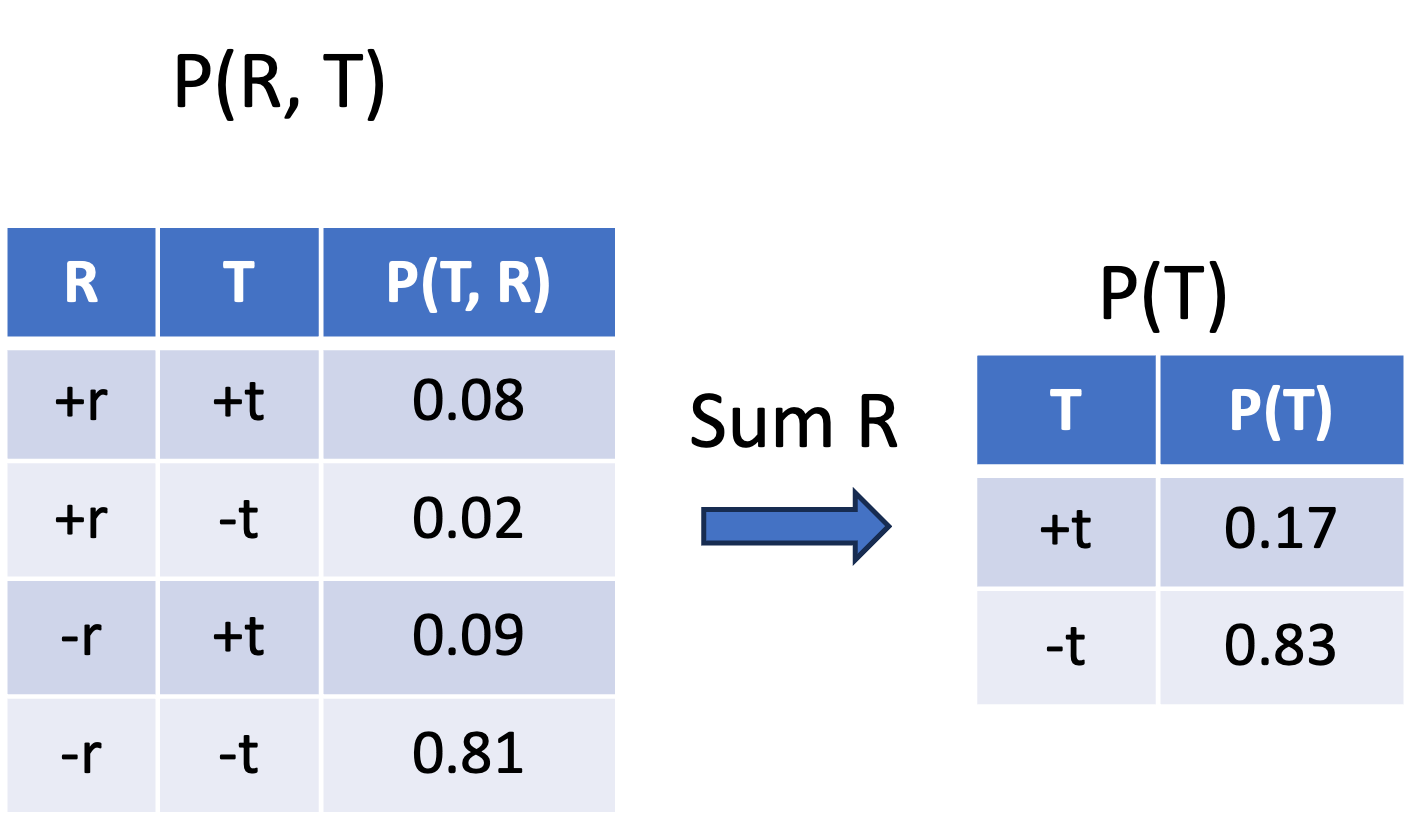
\includegraphics[width=8cm, height = 4cm]{op2_eli.png}

            \item Example2: Multiple elimination
            
            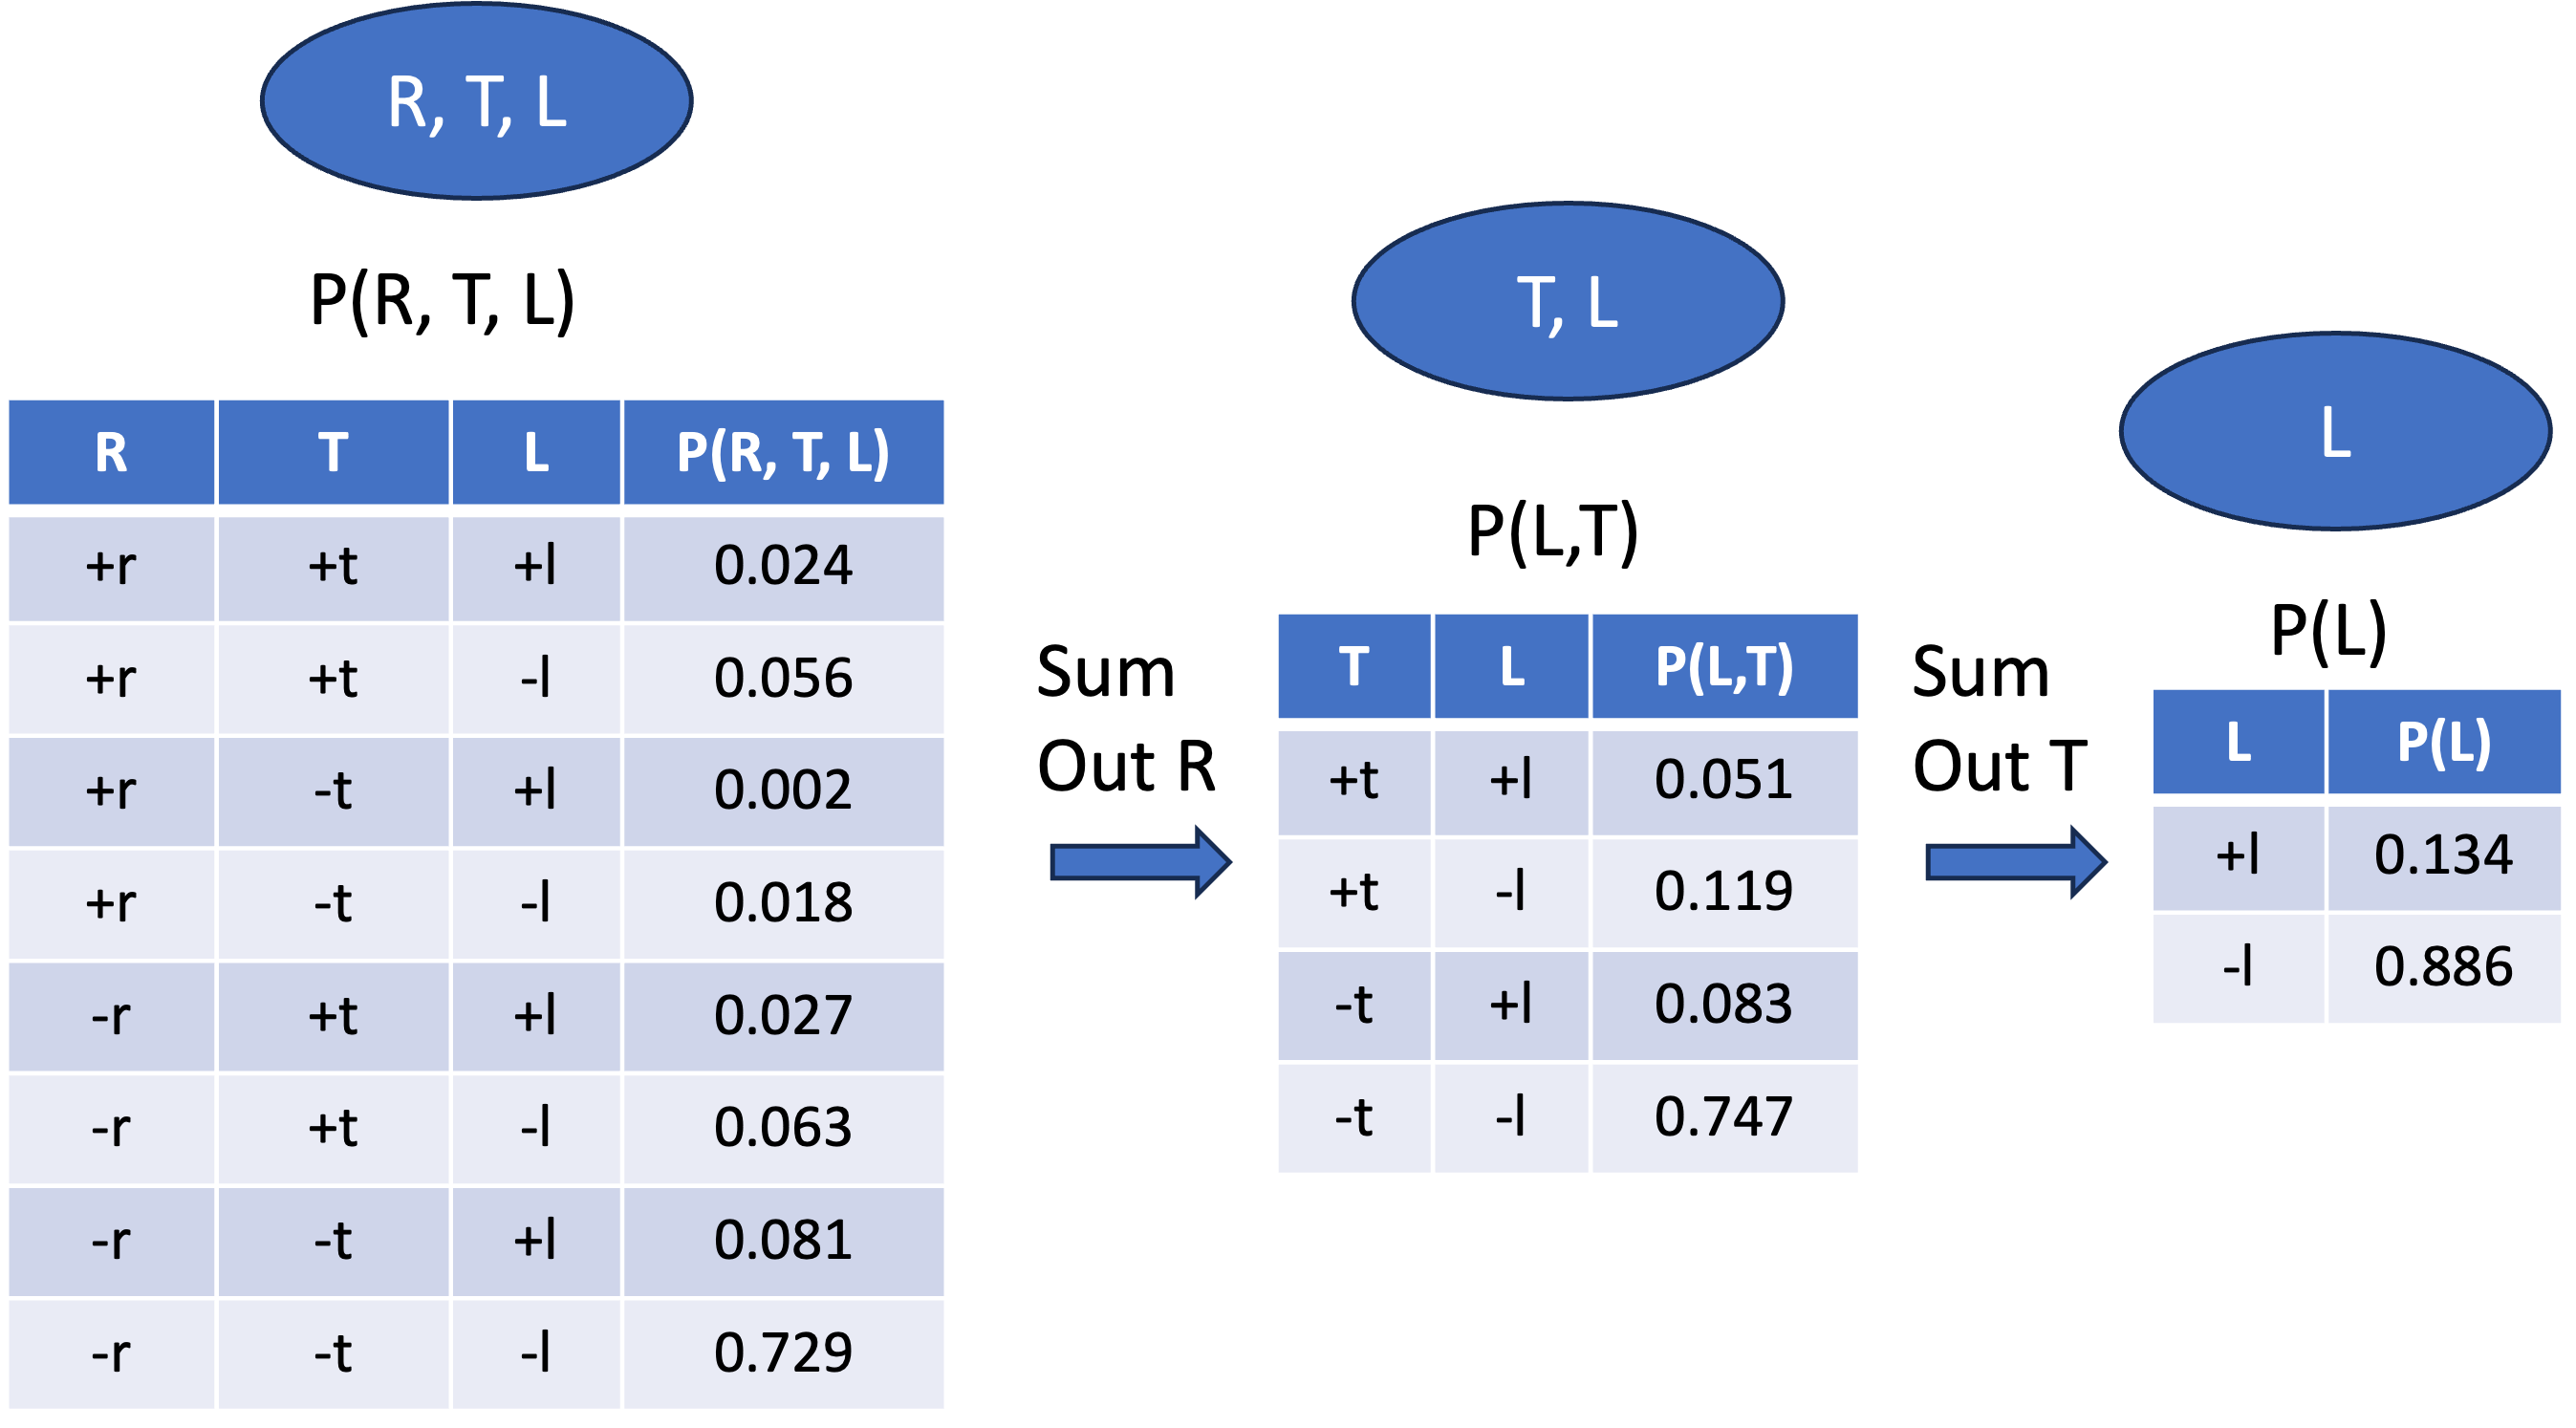
\includegraphics[width=14cm, height = 6cm]{op2_meli.png}
        \end{itemize}
\end{itemize}

\section{Variable Elimination: Marginalize Early!}

You cannot marginalize a variable until you join all factors that include that variable. Except for query variable, which is to leave to the end. For evidential variables, we select them at the first step. 
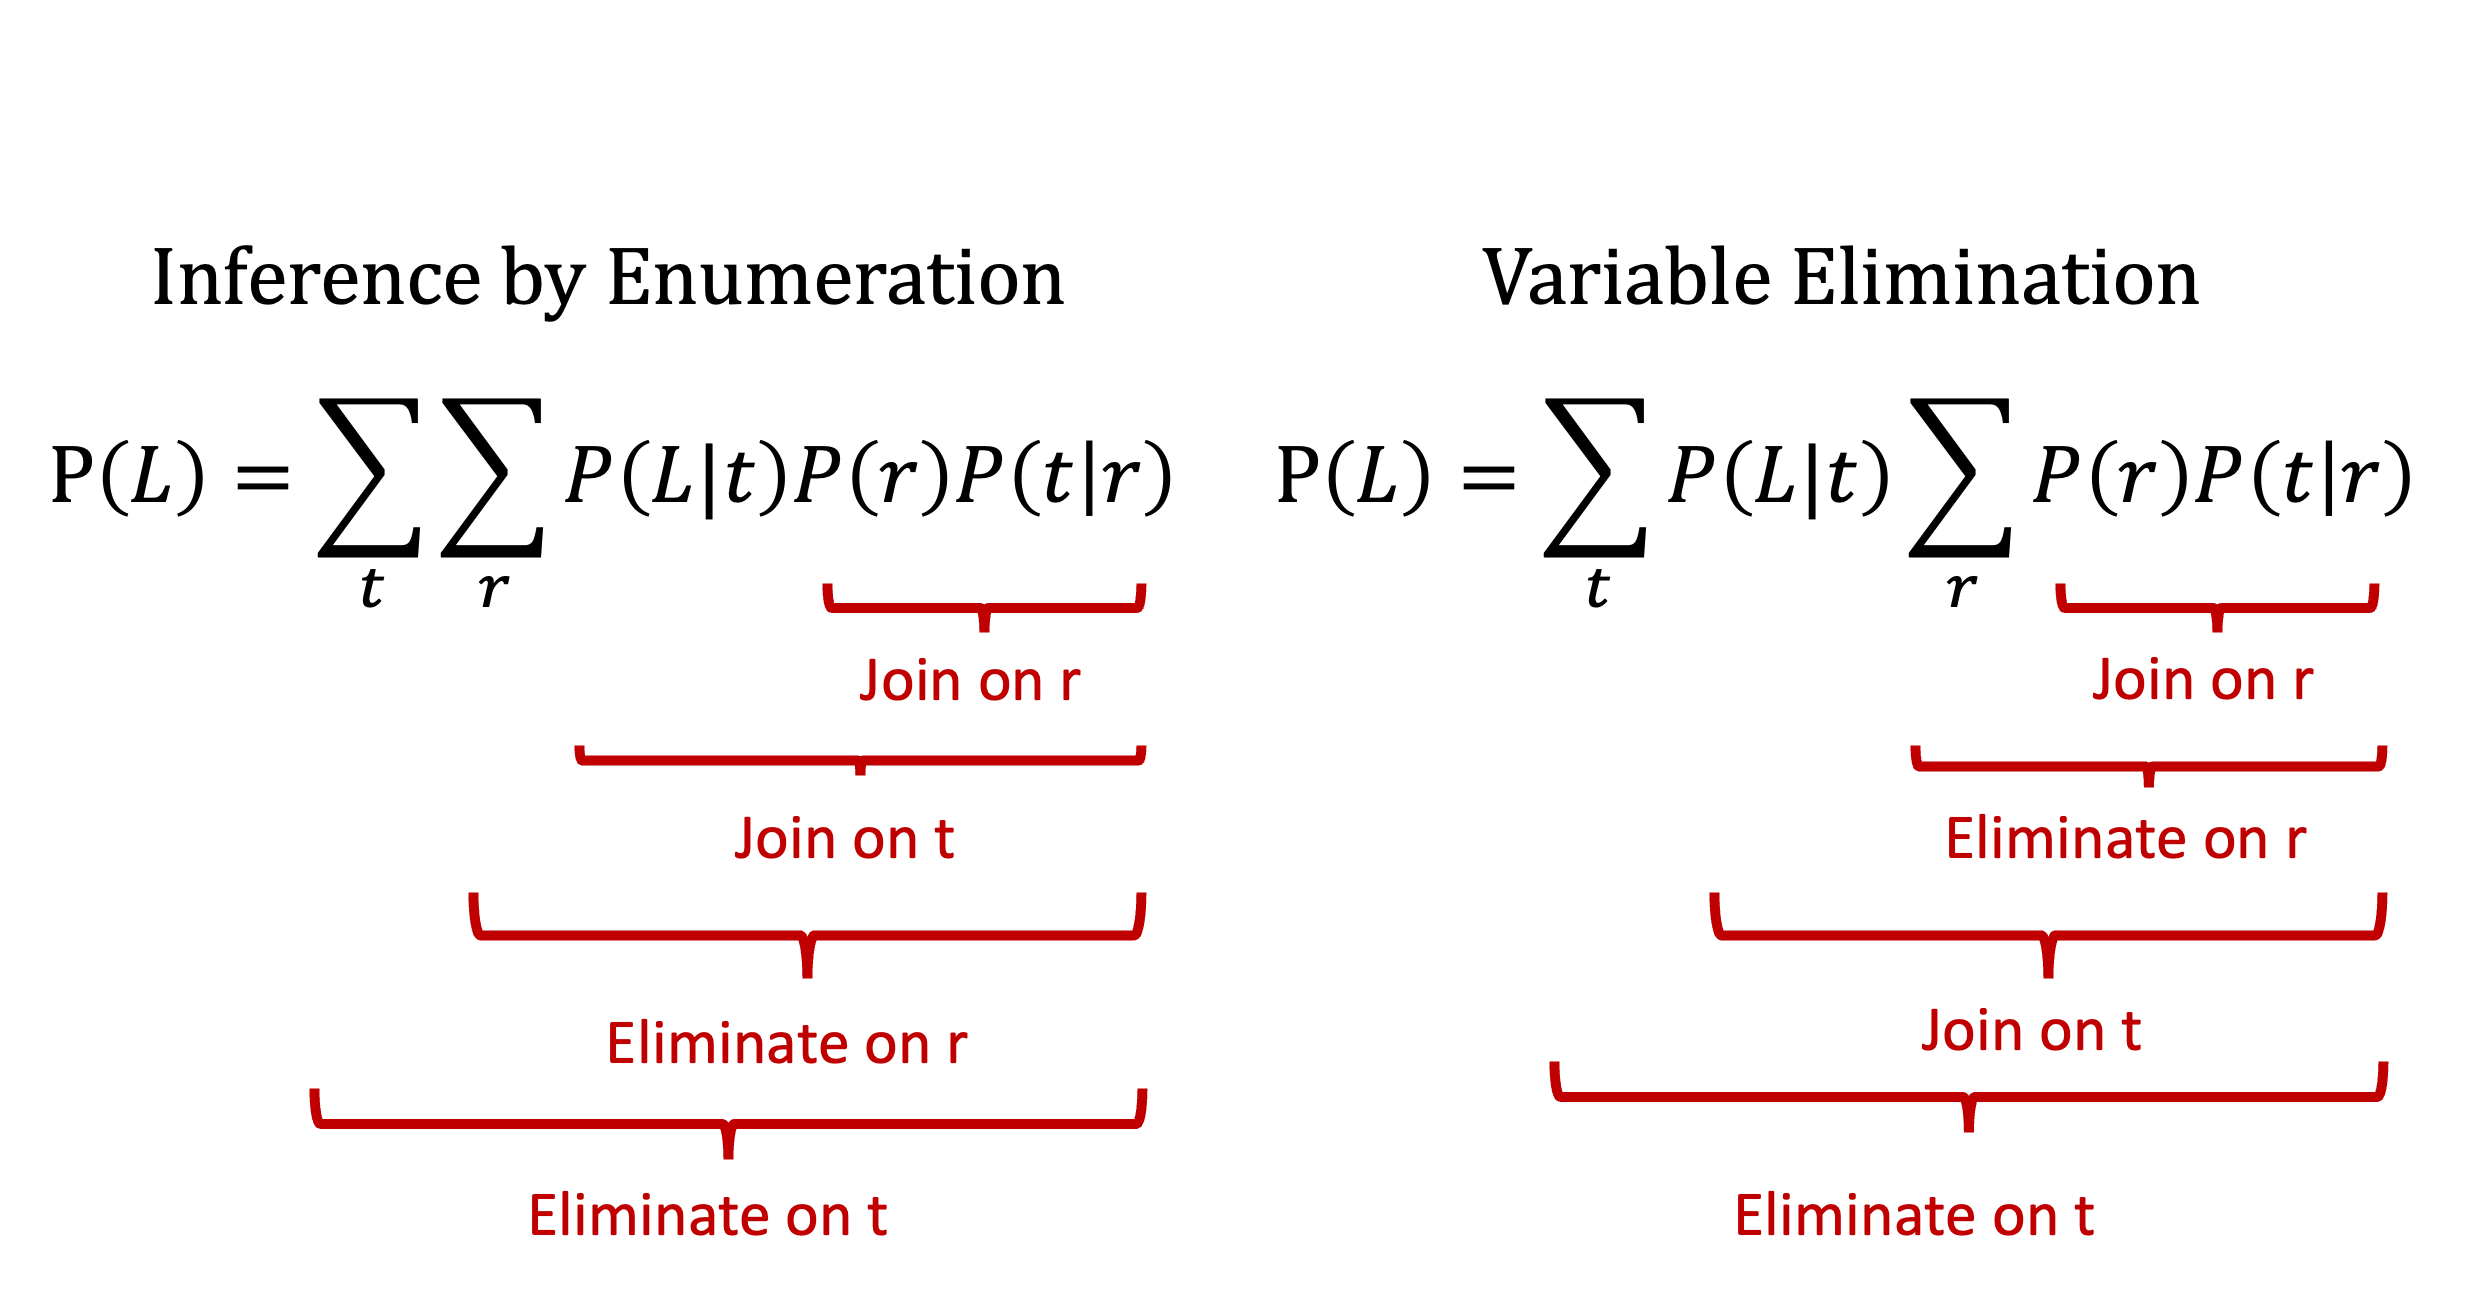
\includegraphics[width=12cm, height = 6cm]{traffic_eg2.png}

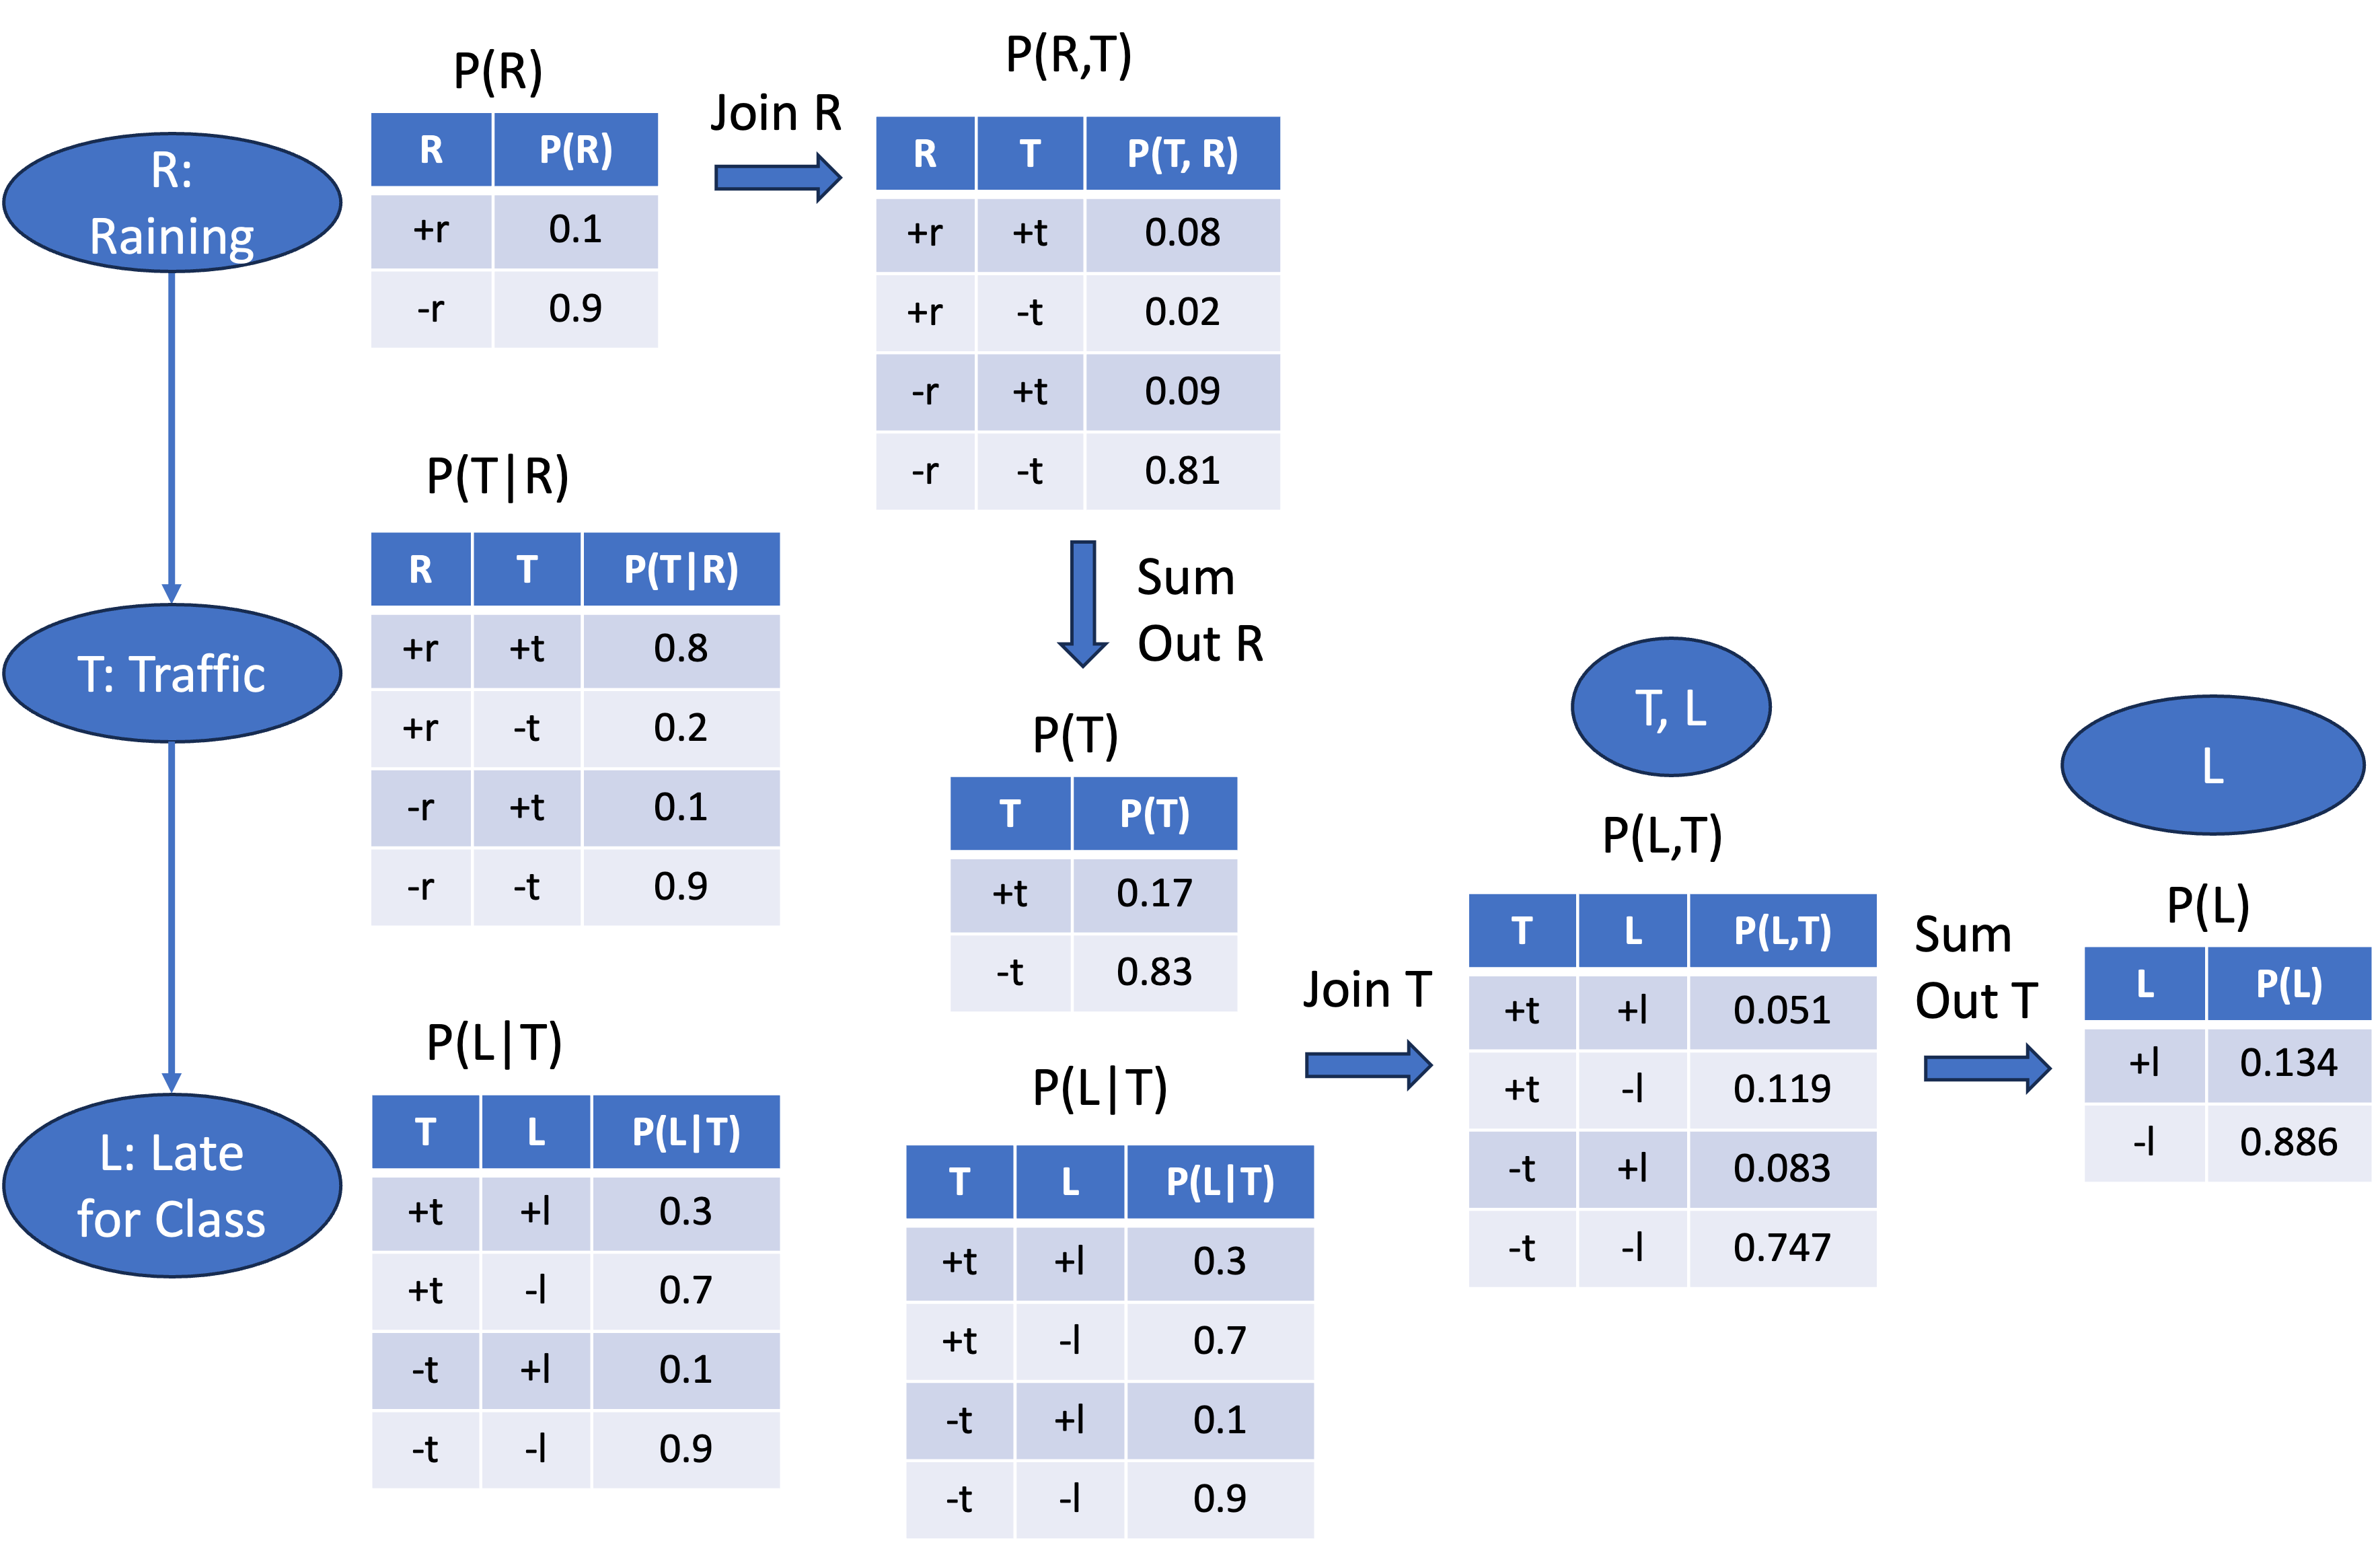
\includegraphics[width=14cm, height = 9cm]{traffic_eg3.png}

\section{Evidence}

\begin{itemize}
    \item If evidence, start with factors that select that evidence
    \begin{itemize}
        \item If there is no evidence, start with following initial factors
        
        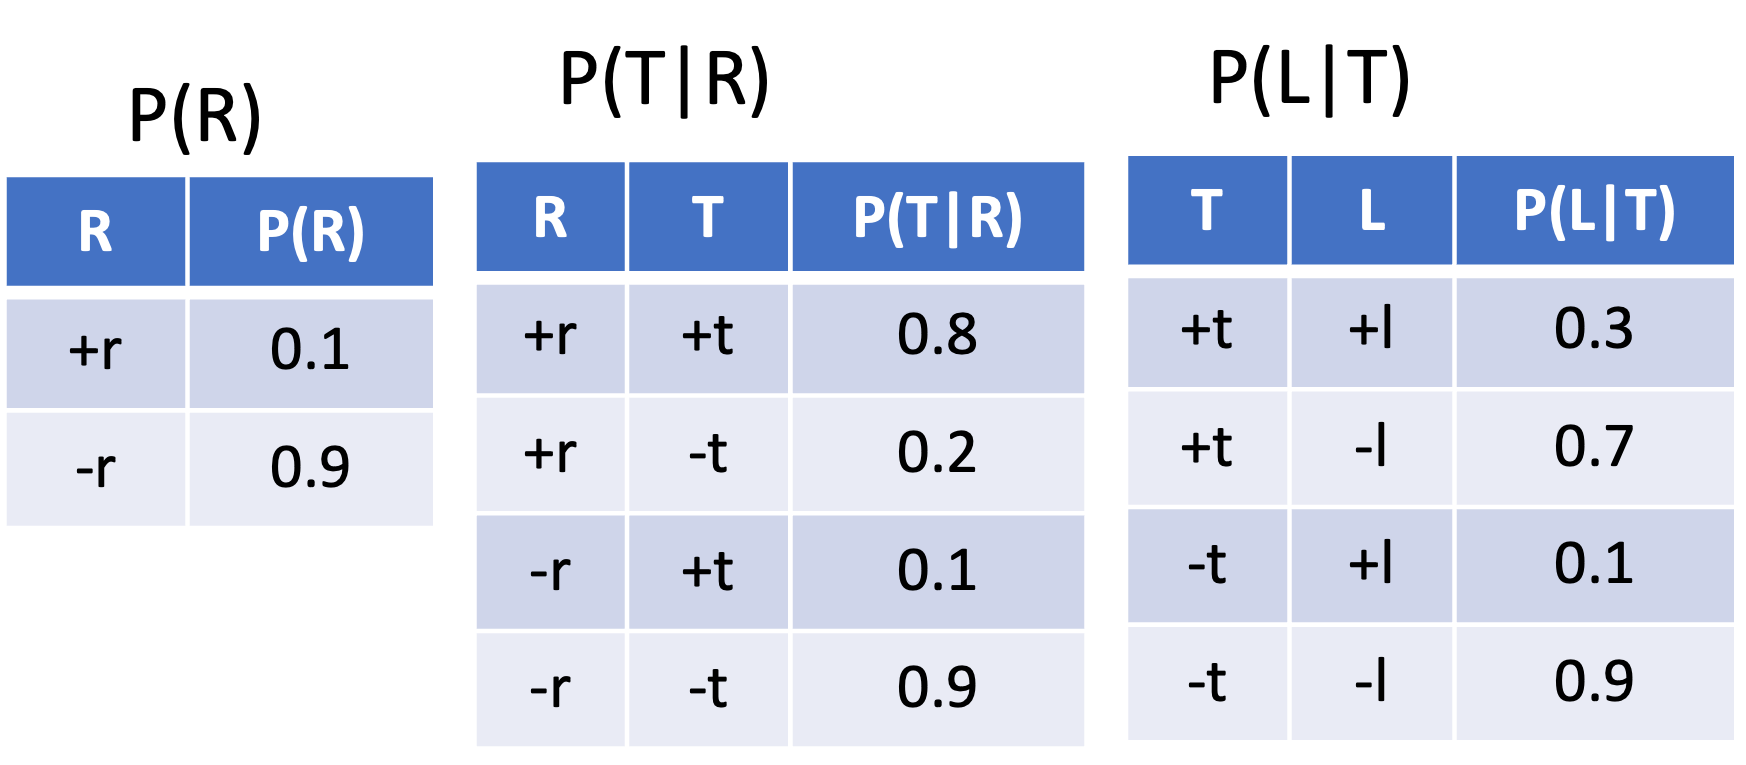
\includegraphics[width=10cm, height = 4cm]{no_evidence.png}

        \item If there is evidence (R = +r), initial factors become
        
        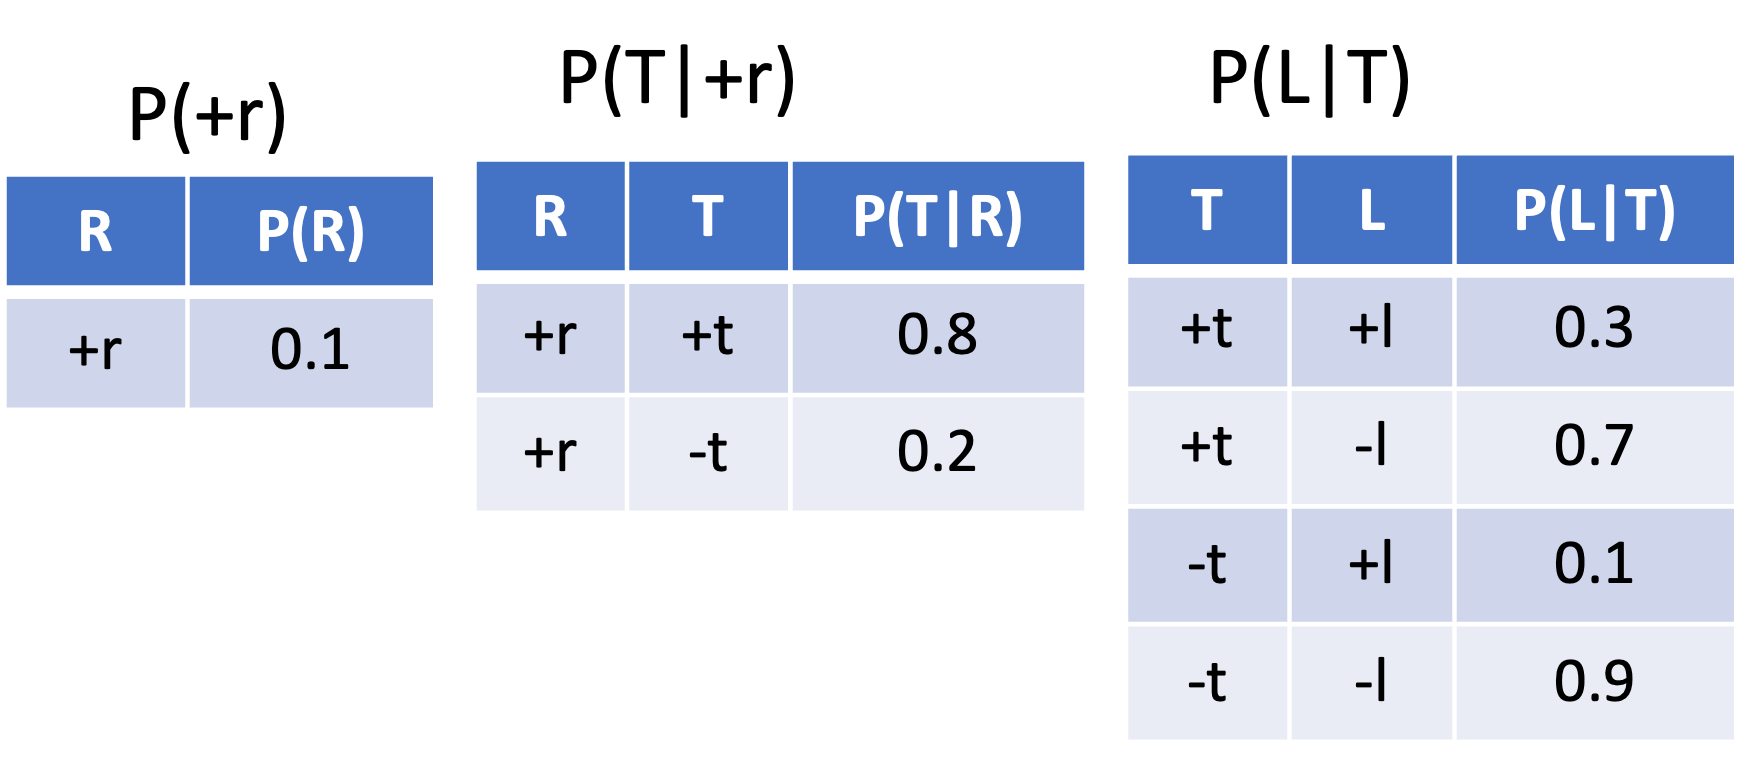
\includegraphics[width=10cm, height = 4cm]{evidence.png}
    \end{itemize}

    \item We eliminate all vars other than query + evidence
    \item Results will be a selected join of query and evidence, to get our answer, normalize it.
    
    For P(L, +r), we would end up with:

    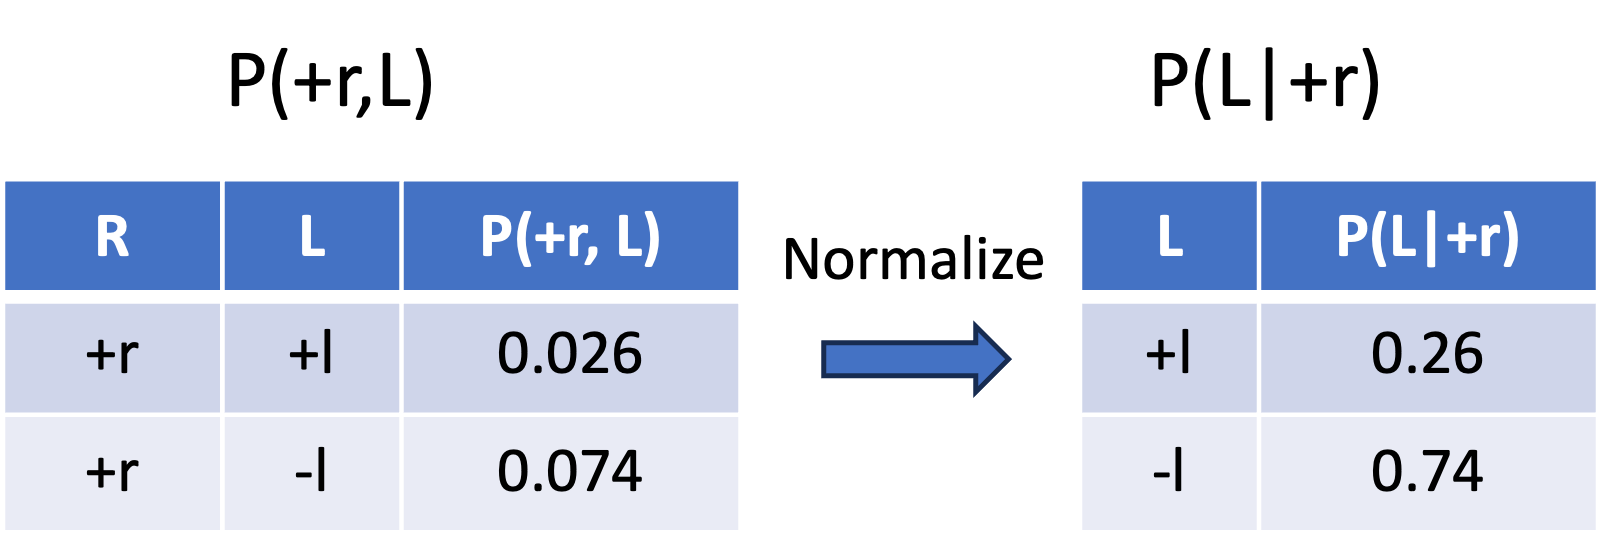
\includegraphics[width=10cm, height = 3cm]{evidence_res.png}

\end{itemize}

\section{General Variable Elimination}

\begin{itemize}
    \item Query: $P(Q \mid E_{1} = e_{1}, \ldots, E_{k} = e_{k})$
    \item Start with initial factors: local CPTs initiated by evidence
    \item While there are still hidden variables:
        \begin{itemize}
            \item Pick a hidden variable H
            \item Join all factors mentioning H
            \item Eliminate (sum out) H
        \end{itemize}
    \item Join all remaining factors and normalize
\end{itemize}

\section{Variable Elimination Ordering}


For the query $P(X_{n} \mid y_{1}, y_{2}, \ldots, y_{n})$ work through the following two different orderings: $Z, X_{1}, X_{2}, \ldots, X_{n-1}$ and $X_{1}, X_{2}, \ldots, X_{n-1}, Z$

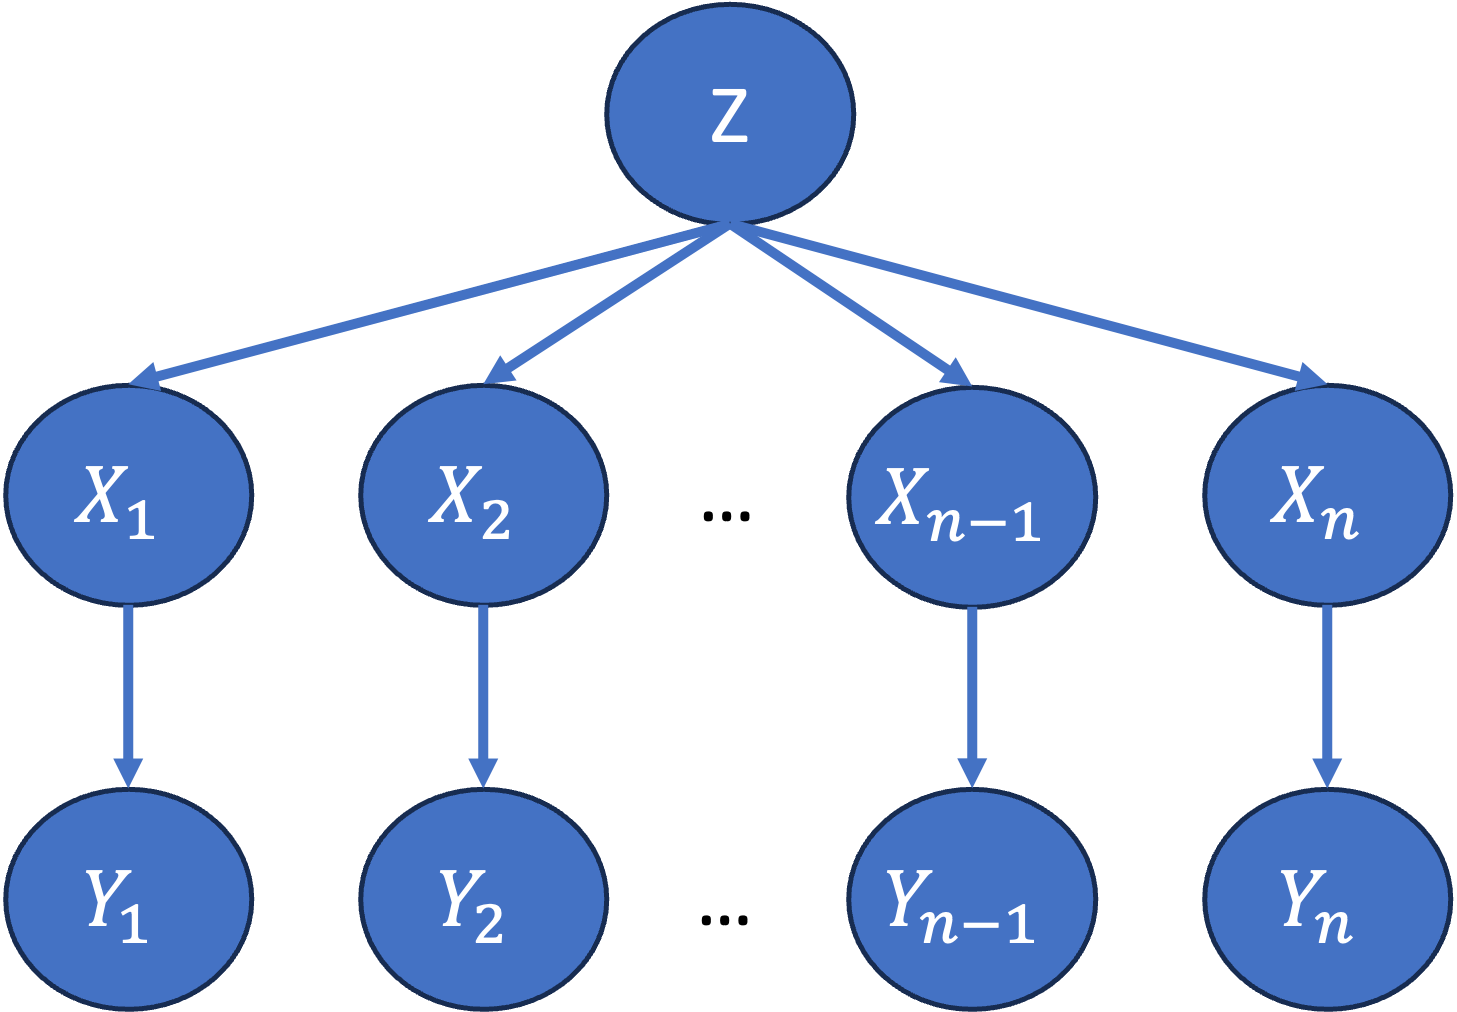
\includegraphics[width=10cm, height = 5cm]{ordering.png}

\begin{itemize}
    \item If we start with $X_{1}$, we need to join $P(Y_{1} \mid X_{1}), P(X_{1} \mid Z)$.
    \item If we start with Z, we need to join $P(Z), P(X_{1} \mid Z), P(X_{2} \mid Z), \ldots, P(X_{n-1} \mid Z)$ (a giant factor).
    \item To find the best ordering: NP-hard
\end{itemize}

\section{Variable Elimination Complexity}

\begin{itemize}
    \item The computational and space complexity of variable elimination is determined by the largest factor.
    \item The elimination ordeing could greatly affect the size of the largest factor. Eg. in previous example, $2^{n}\ vs\ 2$
    \item Factor size: $d^{k}$ entries calculated for a factor over k variables with domain size d.
    \item Does there always exist an ordering that only results in small factors? NO. 
    \item Worst case: running time exponential in the size of the BN.
    \item Inference in BN is NP-hard. No known efficient probabilistic inference in general.
    \item Good situation: Polytree
        \begin{itemize}
            \item A polytree is a directed graph with no undirected cycles.
            \item For polytrees, you can always find an ordering that is efficient.
            \item Choose set of variables that if removed only a polytree remains.
        \end{itemize}
    
\end{itemize}

%%------------------------------- chapter ------------------------------------

\chapter{Sampling}

\section{Approximate Inference: Sampling}

Trade off: Computation versus Accuracy.

\begin{itemize}
    \item Sampling is a lot like repreated simulation. Sampling could be used for learning (we do not know the real probability distribution, but we could interact with the world to learn). However, here we use sampling for inference. We know probabilities and we sample for faster computation.
    
    \item Why sample?
        \begin{itemize}
            \item Learning: get samples from a distribution you do not know.
            \item Inference: get a sample is faster than computing the right answer.
        \end{itemize}

    \item Basic Idea
        \begin{itemize}
            \item Draw N samples from a sampling distribution S
            \item Compute an approximate posterior probability
            \item Show this converges to the true probability P.
        \end{itemize}

    \item Sampling from Given Distribution
        \begin{itemize}
            \item Step1: given sample u from uniform distribution over $\left[0, 1 \right)$. eg: random() in python
            \item Step2: convert this sample u into an outcome for the given distribution by having each target outcome associated with a sub-interval of $\left[0, 1 \right)$ with sub-interval size equal to probability of the outcome.
            
            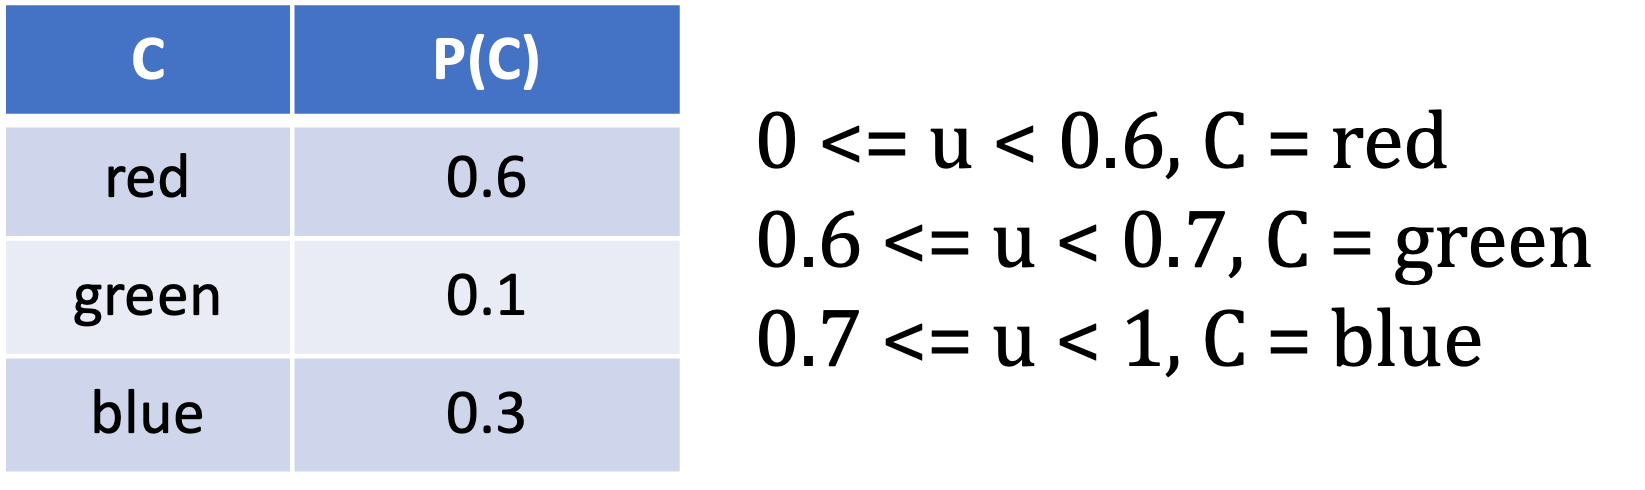
\includegraphics[width=10cm, height = 3cm]{sampling.png}
        \end{itemize}
\end{itemize}

\section{Prior Sampling}

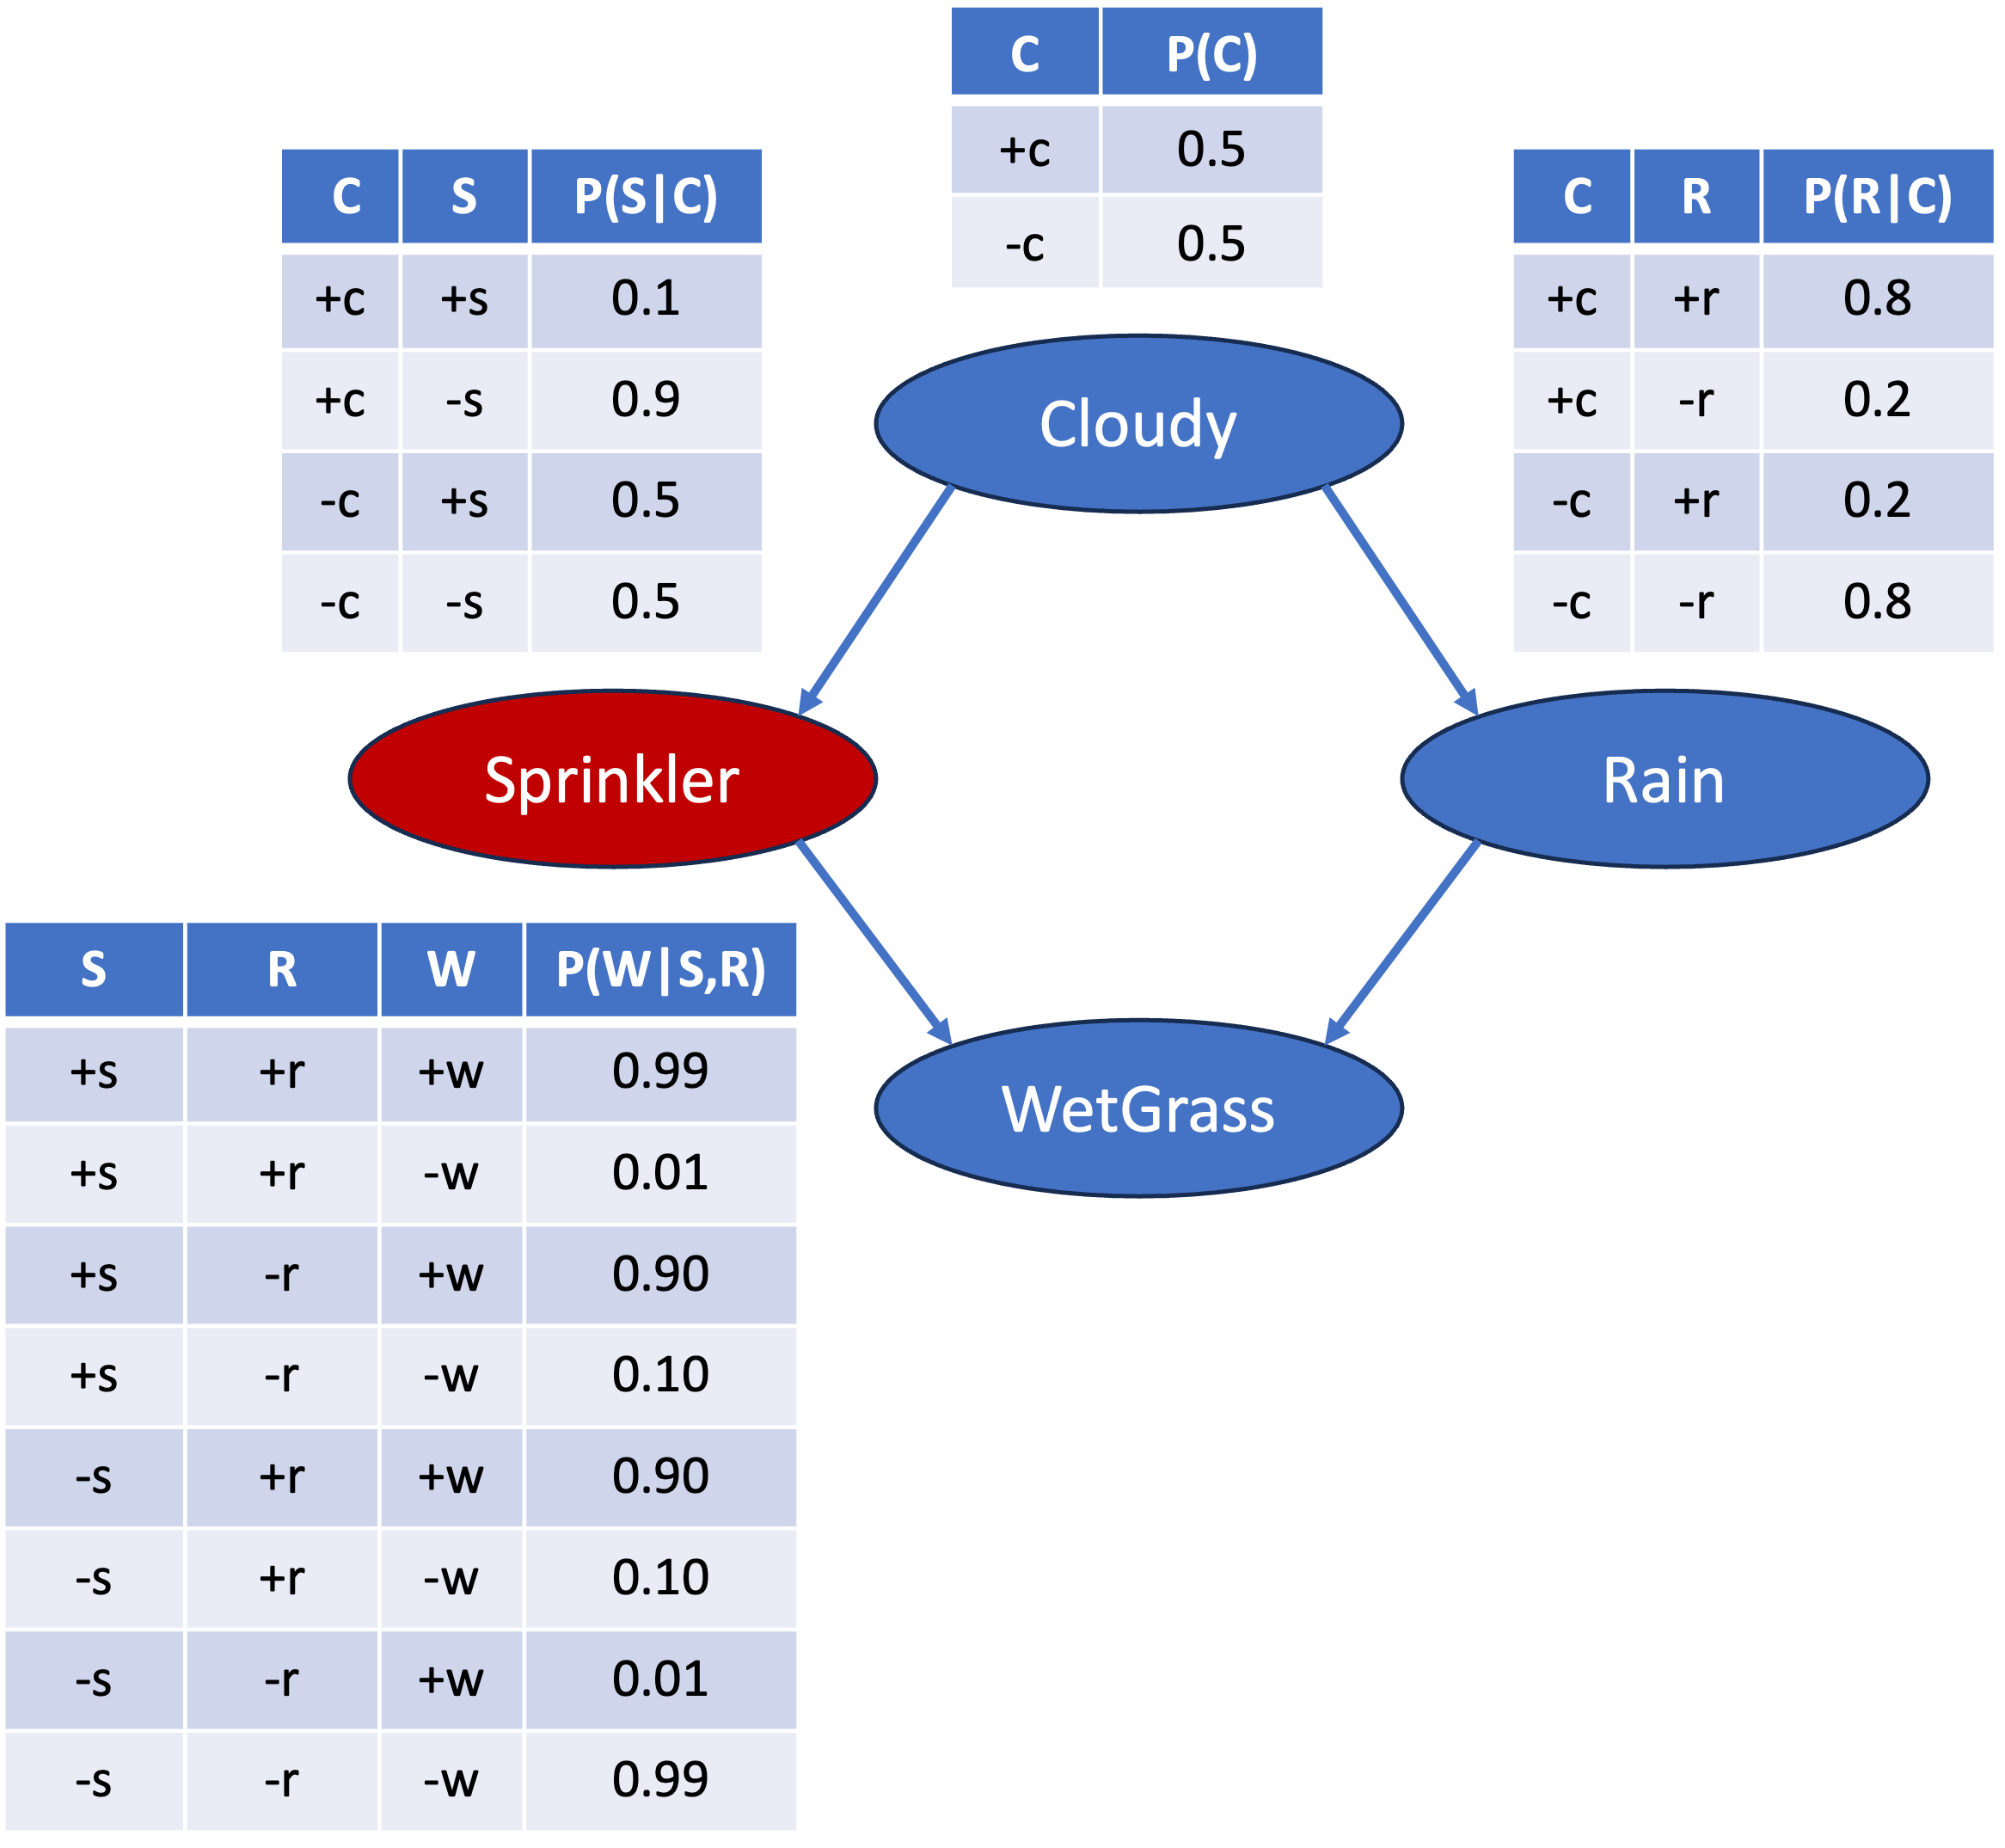
\includegraphics[width=12cm, height = 10cm]{sampling_prior.png}

\begin{itemize}
    \item For i = 1, 2, \ldots, n, \\
        sample $x_{i}$ from $P(X_{i} \mid Parents(X_{i}))$. \\
    
    Return $(x_{1}, x_{2}, \ldots, x_{n})$
    \item This process generates samples with probability
        \begin{center}
            $S_{PS}(x_{1}, x_{2},\ldots, x_{n}) = \prod_{i=1}^{n} P(x_{i} \mid Parents(X_{i})) = P(x_{1}, x_{2}, \ldots, x_{n})$
        \end{center}
    \item Let the number of samples of an event be $N_{PS}(x_{1}, x_{2}, \ldots, x_{n})$
    \item Then,
        \begin{center}
            \begin{equation}
                \begin{split}
                    \lim_{x \to \infty} P(x_{1}, \ldots, x_{n}) & =  \lim_{x \to \infty} \frac{N_{PS}(x_{1}, x_{2}, \ldots, x_{n})}{N} \\
                    & = S_{PS}(x_{1}, x_{2}, \ldots, x_{n}) \\
                    & = P(x_{1}, x_{2}, \ldots, x_{n}) \\
                \end{split}
            \end{equation}
        \end{center}
    \item The sampling procedure is consistent (the sampling distribution approximate the actual distribution).
    \item Example
        \begin{itemize}
            \item We will get a bunch of samples from the BN \\
                    +c, -s, +r, +w \\
                    +c, +s, +r, +w \\
                    -c, +s, +r, -w \\
                    +c, -s, +r, +w \\
                    -c, -s, -r, +w \\
            \item If we want to know P(W)
                \begin{itemize}
                    \item We have counts <+w:4, -w:1>
                    \item Normalize to get P(W) = <+w:0.8, -w:0.2>
                    \item This will get closer to the true distribution with more samples.
                    \item What about P(C|-r,-w)? we don't have the sample, therefore cannot answer the question.
                    \item Fast: can use fewer samples if less time
                \end{itemize}
        \end{itemize}
\end{itemize}

\section{Rejection Sampling}

\begin{itemize}
    \item We get a bunch of samples from the BN \\
    +c, -s, +r, +w \\
    +c, +s, +r, +w \\
    -c, +s, +r, -w \\
    +c, -s, +r, +w \\
    -c, -s, -r, +w \\
    \item Lets say we want P(C|+s)
    \item Tally C outcomes, but reject samples which do not have S = +s. This is called rejection sampling
    \item It is also consistent for conditional probabilities

    \item For i = 1, 2, \ldots, n, \\
        \begin{itemize}
            \item sample $x_{i}$ from $P(X_{i} \mid Parents(X_{i}))$. \\
            \item if $x_{i}$ not consistent with evidence, \\
                reject: return no sample generated in this cycle.
        \end{itemize}

    Return $(x_{1}, x_{2}, \ldots, x_{n})$
\end{itemize}

\section{Likelihood Sampling}

\begin{itemize}
    \item Problems with rejection sampling
        \begin{itemize}
            \item If evidence is unlikely, reject lots of samples
            \item Evidence is not exploited
        \end{itemize}
    
    \item Idea: fix evidence variables and sample the rest
        \begin{itemize}
            \item Problem: sample distribution not consistent (eg, we assume that all sampling obects are blue. The probability of P(blue) changed to 1.)
            \item Solution: weight by probability of evidence given parents.
        \end{itemize}
    
    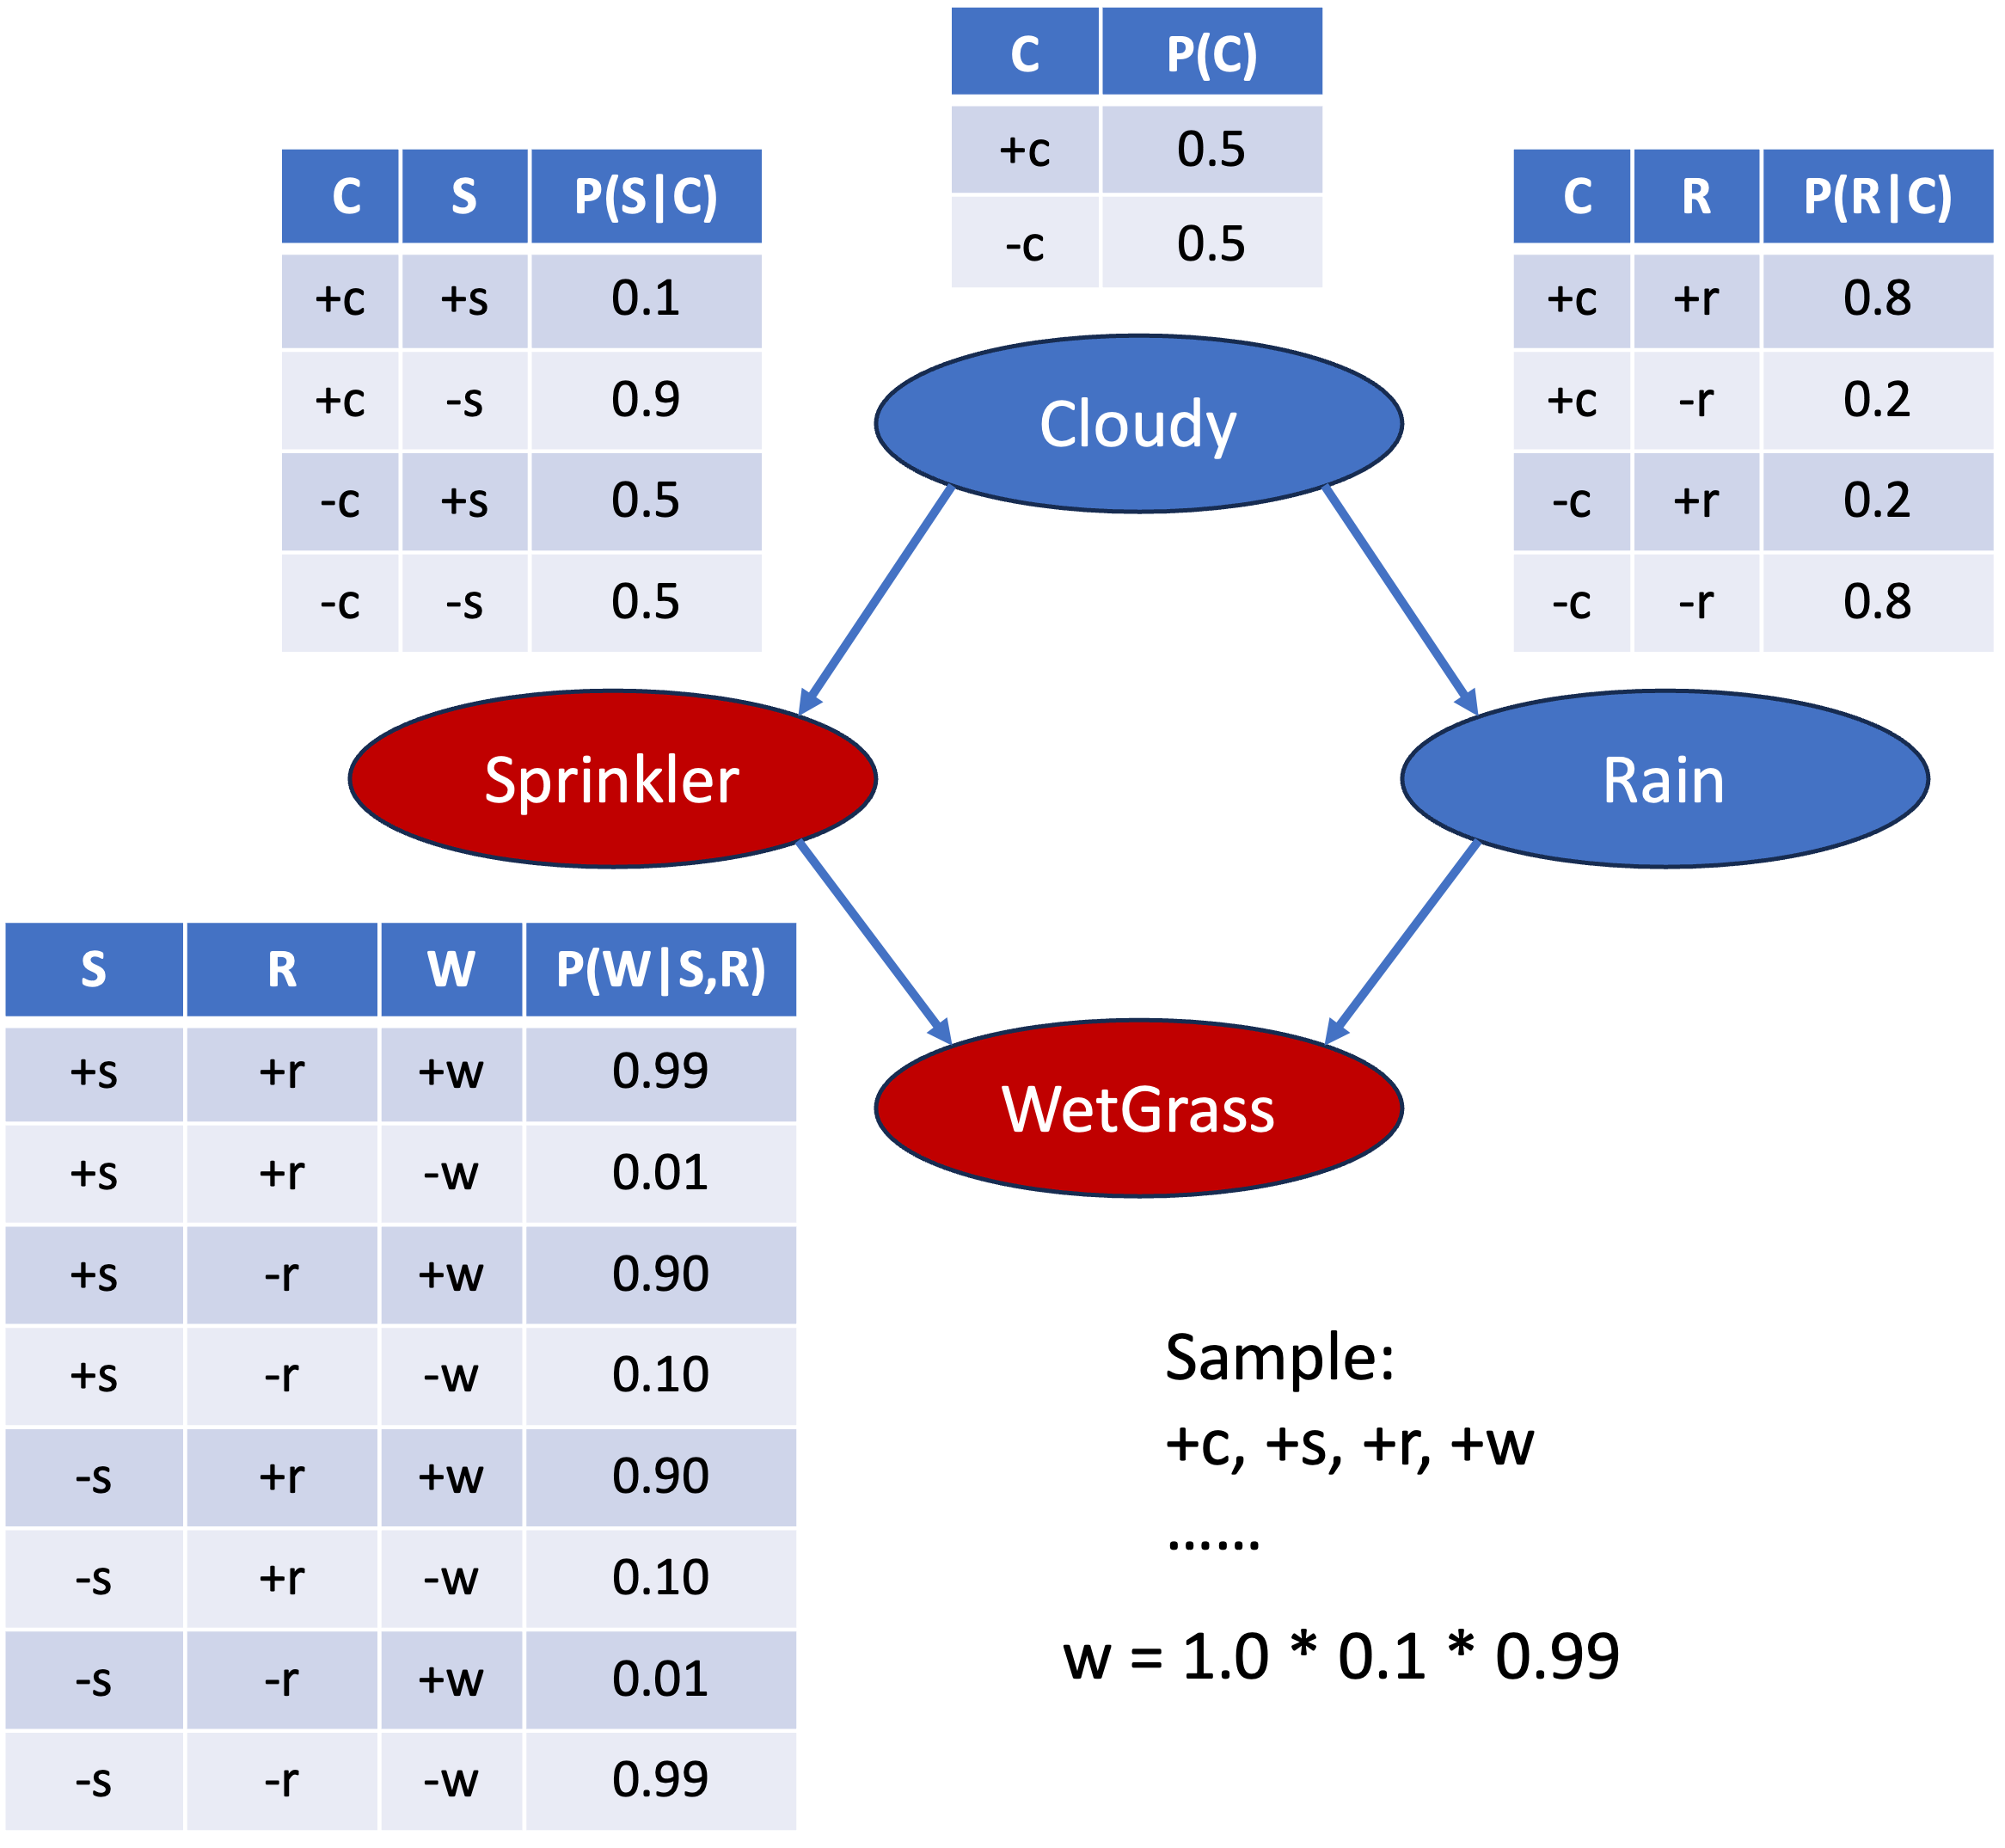
\includegraphics[width=12cm, height = 10cm]{sampling_likelihood.png}

    \item Algorithm
        \begin{itemize}
            \item input: evidence initiation
            \item w = 1.0
            \item for i = 1, 2, \ldots, n, \\
               \begin{itemize}
                    \item if $X_{i}$ is an evidence variable
                        \begin{itemize}
                            \item $x_{i}$ = obeservation $x_{i}$ for $X_{i}$
                            \item Set w = w * $P(x_{i} \mid Parents(X_{i}))$
                        \end{itemize}
                    \item else:
                        \begin{itemize}
                            \item sample $x_{i}$ from $P(X_{i} \mid Parents(X_{i}))$.
                        \end{itemize}
                \end{itemize}
            \item Return $(x_{1}, x_{2}, \ldots, x_{n}), W$
        \end{itemize}
    
    \item Sampling distribution if z sampled and e fixed evidence
    \begin{center}
        $S_{W S}(z, e) = \prod_{i=1}^{l}P(Z_{i} \mid Parents(Z_{i}))$
    \end{center}
    \item Now, samples have weights
    \begin{center}
        $w(z, e) = \prod_{i=1}^{m}P(e_{i} \mid Parents(E_{i}))$
    \end{center}
    \item Together, weighted sampling distribution is consistent
    \begin{center}
        $S_{W S}(z, e) * w(z, e) = \prod_{i=1}^{l}P(Z_{i} \mid Parents(Z_{i})) *  \prod_{i=1}^{m}P(e_{i} \mid Parents(E_{i}))$

        $S_{W S}(z, e) * w(z, e) = P(z, e)$
    \end{center}

    \item Likelihood weighting is good
        \begin{itemize}
            \item We have taken evidence into account as we generate the sample
            \item Most of our samples will reflect the  state of the world suggested by evidence.
        \end{itemize}
    
    \item Likelihood weighting does not solve all problems. Likelihood works well when evidence is at the top. Evidence influences the choices of downstream variables, but not upstream ones. However, if the evidence is at the bottom, for instance, suppose the evidence is we know john called. Likelihood weighting is good at simulating consequences of evidence, but not very good at simulating the causes the evidence.
\end{itemize}

\section{Example}

\begin{itemize}
    \item Prior Sampling
    
    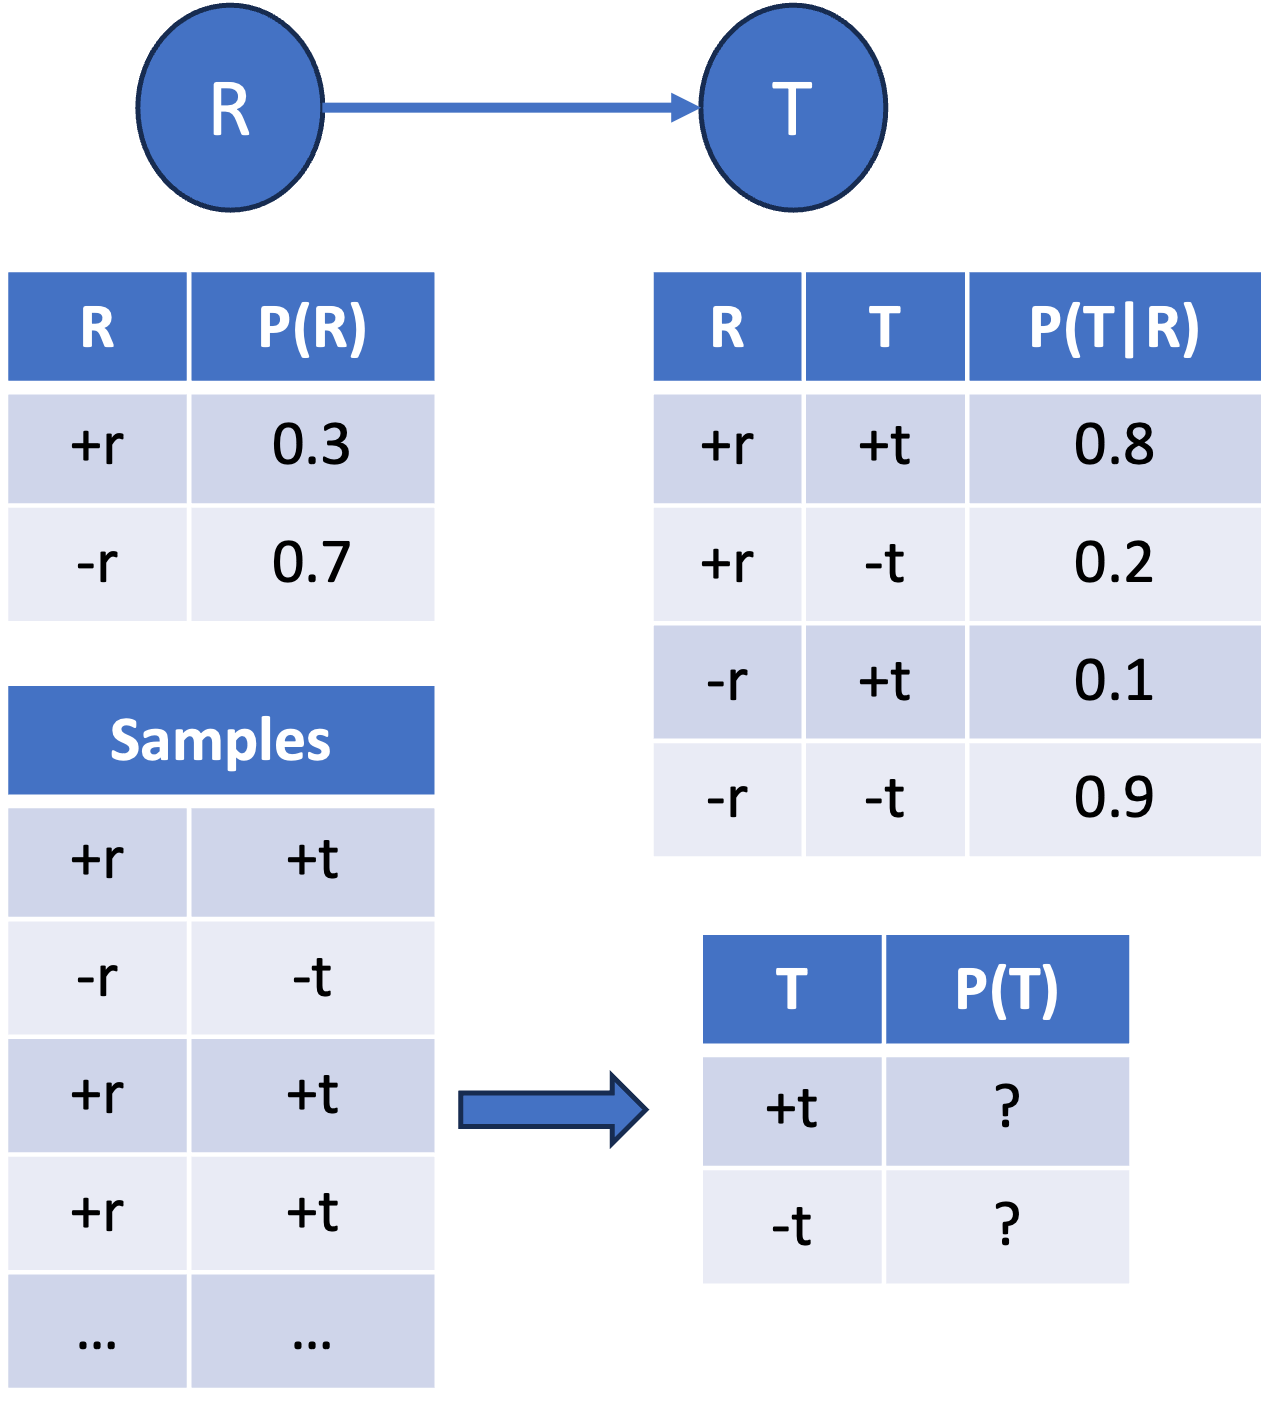
\includegraphics[width=6cm, height=7cm]{sampling_eg_prior.png}\\

    In the sample, p(+t) = $\frac{3}{4}$, it might not be equal to true p(+t). However, it get the 4000 samples, these two numbers will be very close.

    \item Rejection Sampling
    
    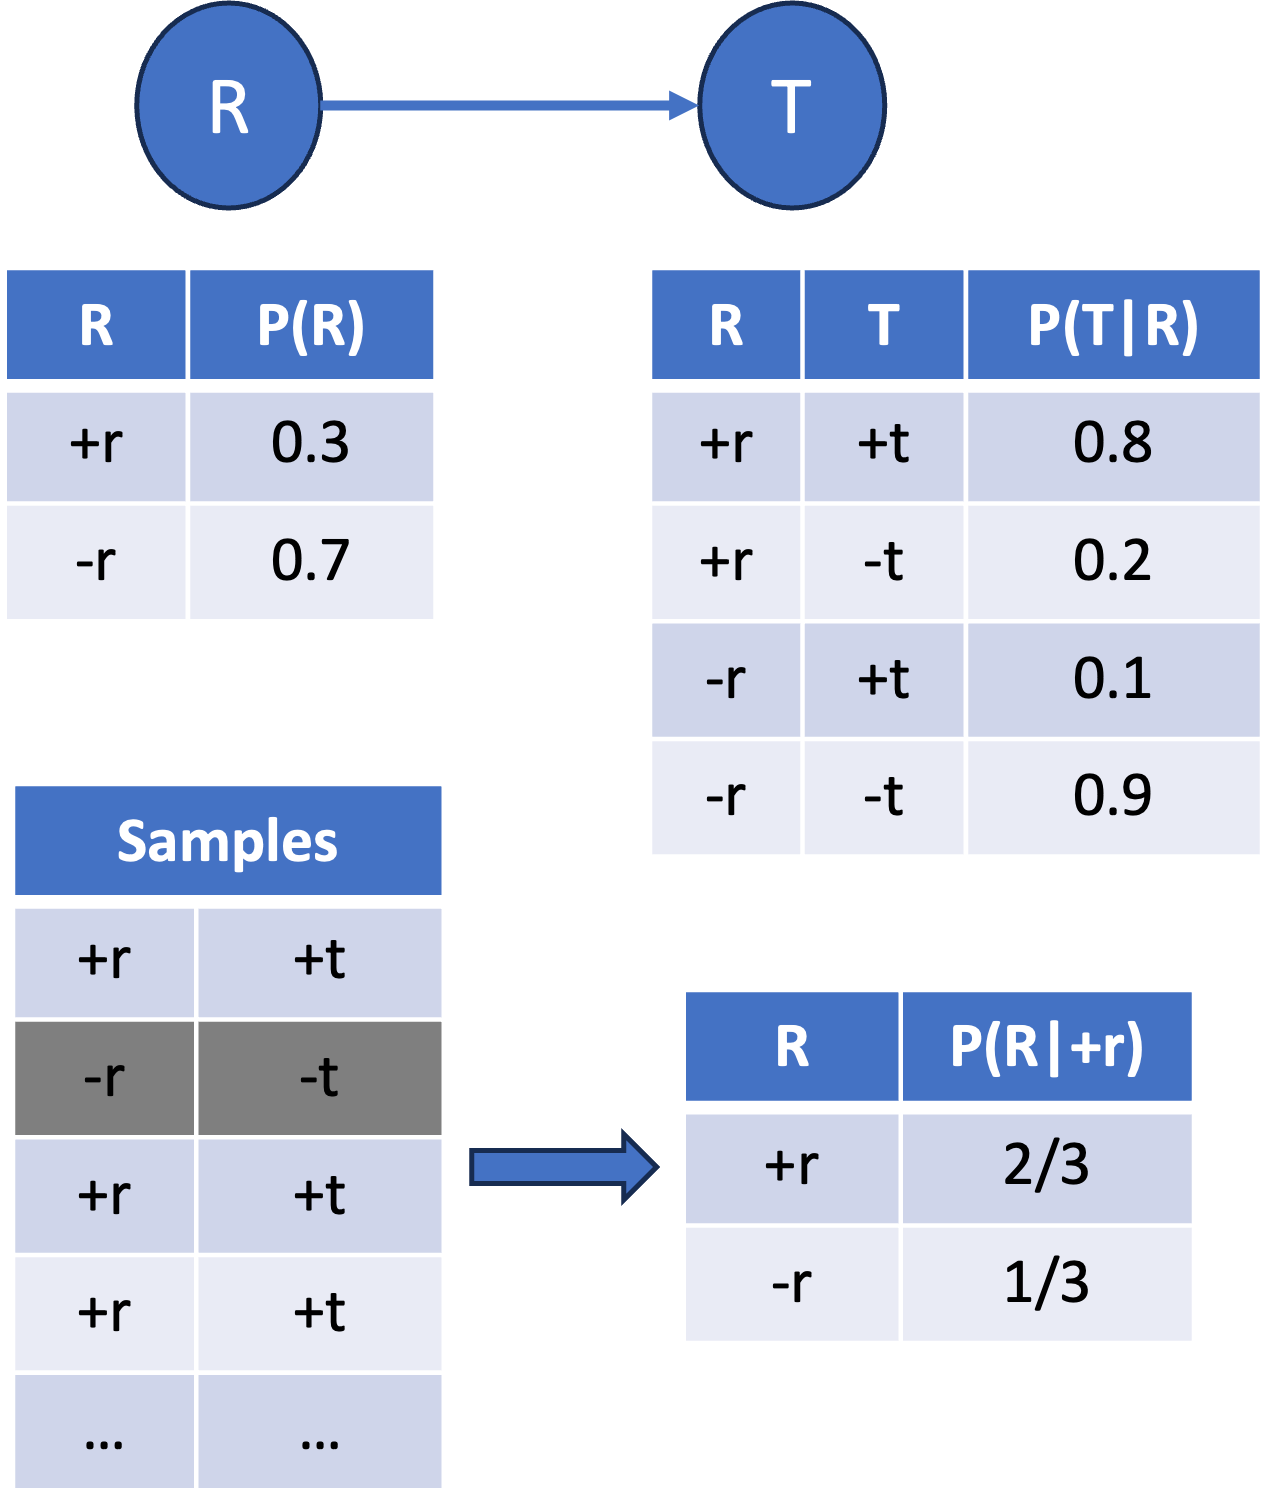
\includegraphics[width=6cm, height=7cm]{sampling_eg_rej.png}\\

    In the sample, p(+t) = $\frac{3}{4}$, We reject one sample T=-t.

    \item Likelihood Weighting
    
    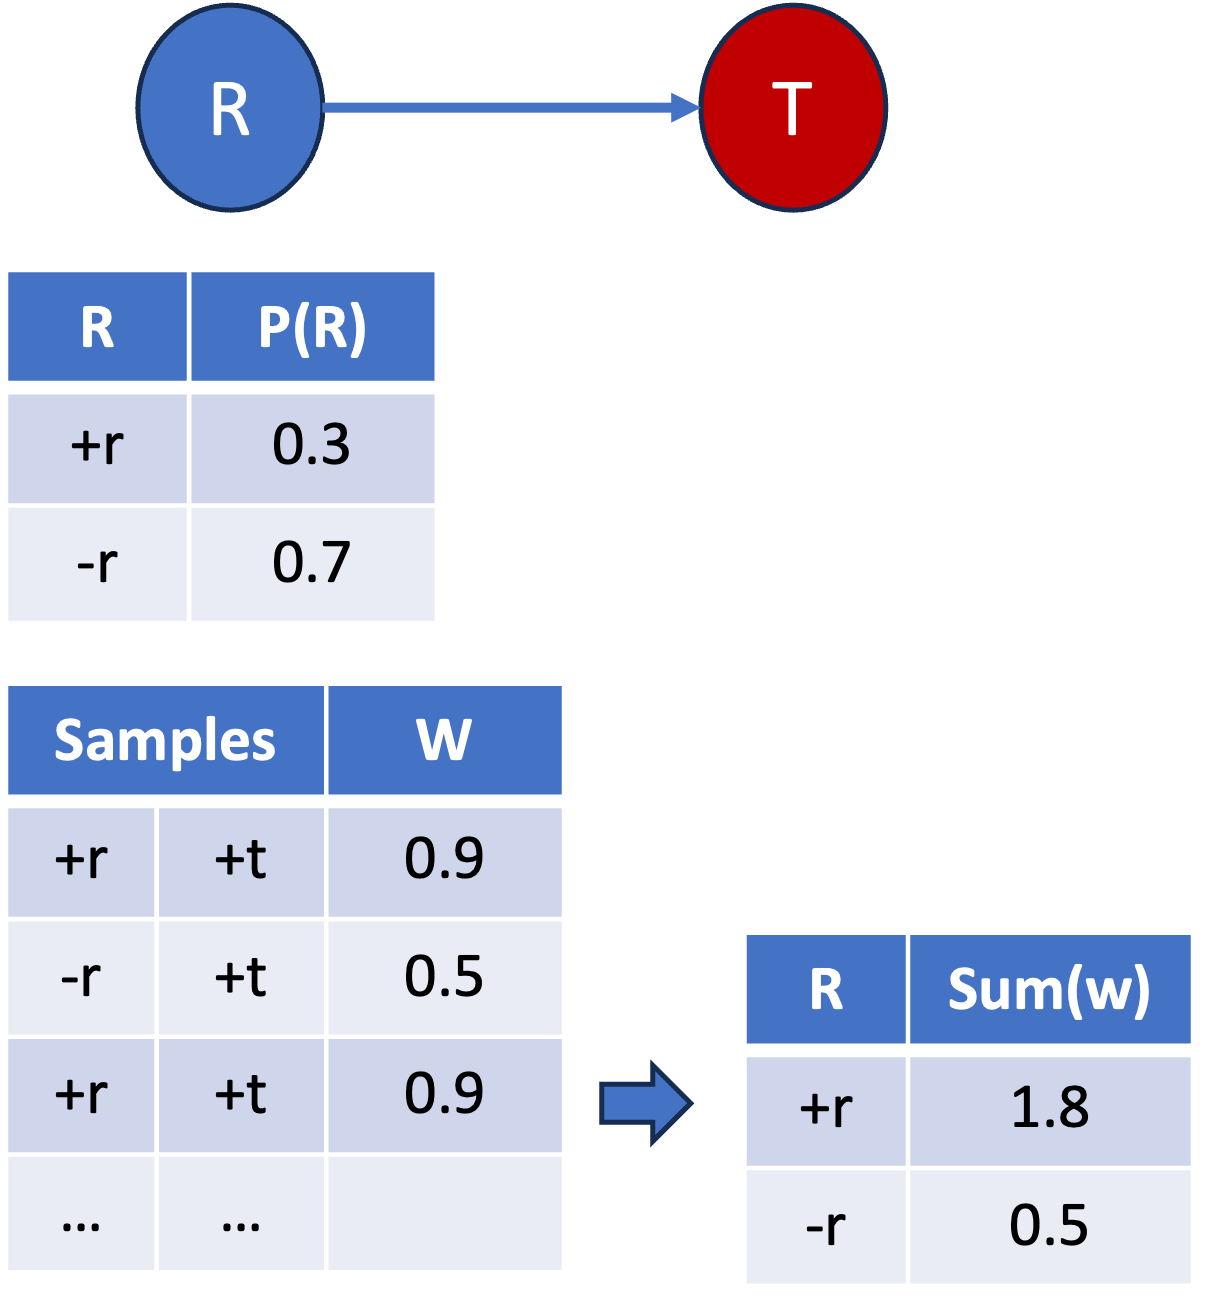
\includegraphics[width=8cm, height = 8cm]{sampling_eg_lik.png}\\

    We do not want to throw away samples, especially when the probability of evidence is small.
    Suppose T is an evidential variable, we know T = +t. Assume in the first sample, we first sample R = +r, normally we would then sample T, since T is evidential variable, we set T = +t, and multiply w by P(T = +t | +r) = 0.9.

    \item Failed Case of Likelihood Weighting

    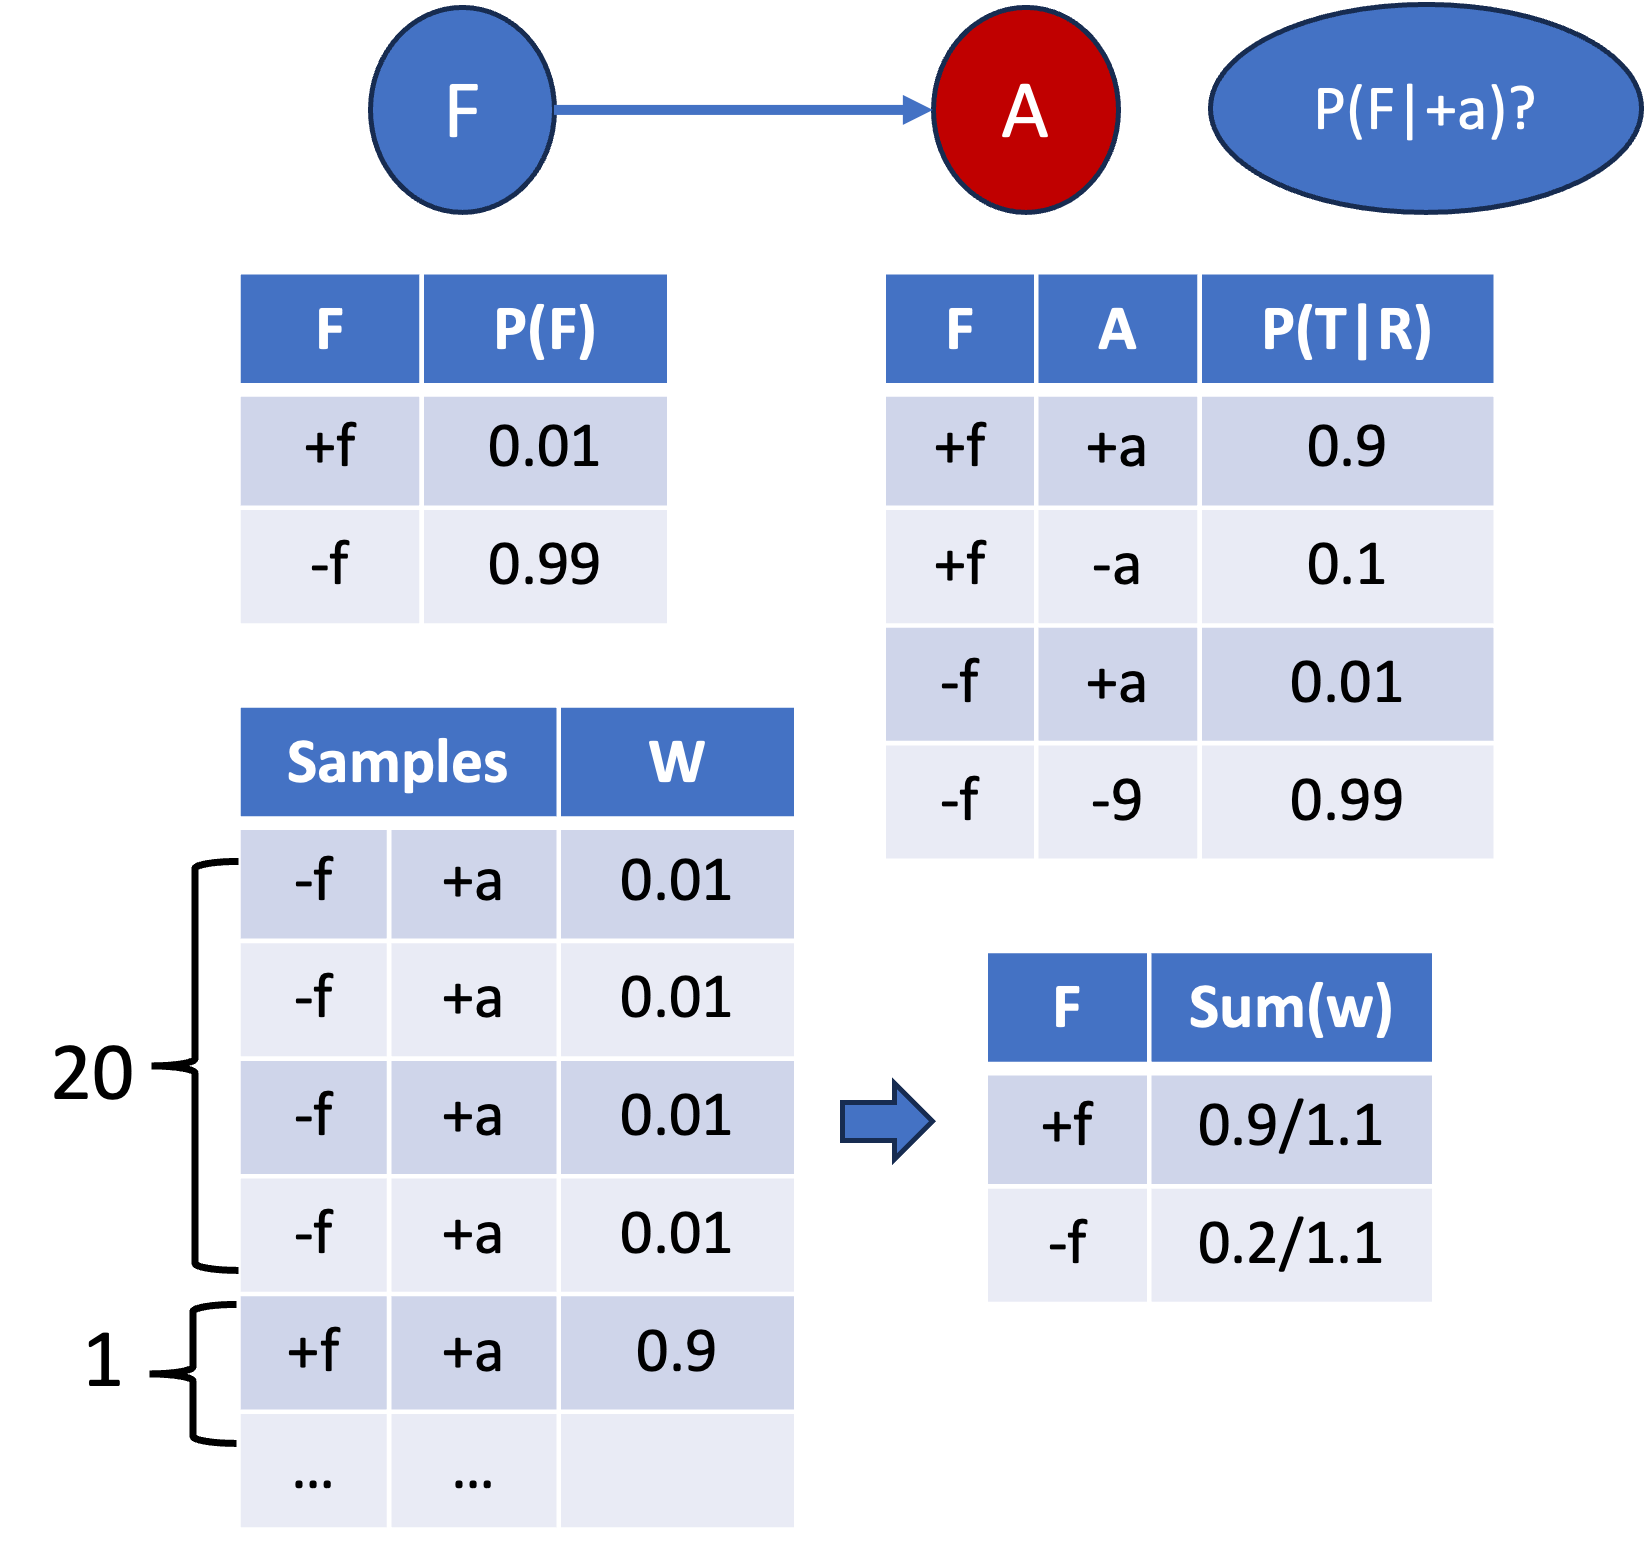
\includegraphics[width=8cm, height = 8cm]{sampling_eg_lik_neg.png}\\

    \begin{itemize}
        \item Failure case of rejection sampling:
        
        If we use reject sampling, we are going to reject lots of samples.

        \item Failure case of Likelihood weighting:
        
        If we use likelihood weighting, we fixed +a, but the weight will be very small. 
        Samples we really need is +f, but it will not happen very often. (but the weight of +f, +a will be very high).
        It will get the right number in the end, but it takes lots of time to generate rare events in the upstream.
    \end{itemize}

\end{itemize}

\section{Gibbs Sampling}

\begin{itemize}
    \item We do not sample from top to the bottom. Instead, we start with a complete assignment. We take into account evidence both upstream and downstream.
    
    \item Procedure: Keep track of a full instantiation $x_{1}, x_{2}, x_{3}, \ldots, x_{n}$. Start with an arbitrary instantiation consistent with the evidence. Sample one variable at a time, conditioned on all the rest, but keep evidence fixed. Keep repeating this for a long time.
    
    \item Rationale: both upstream and downstream variables condition on evidence.
    
    \item In contrast: likelihood weighting only conditions on upstream evidence, and hence weights obtained in likelihood weighting can sometimes be very small.
    
    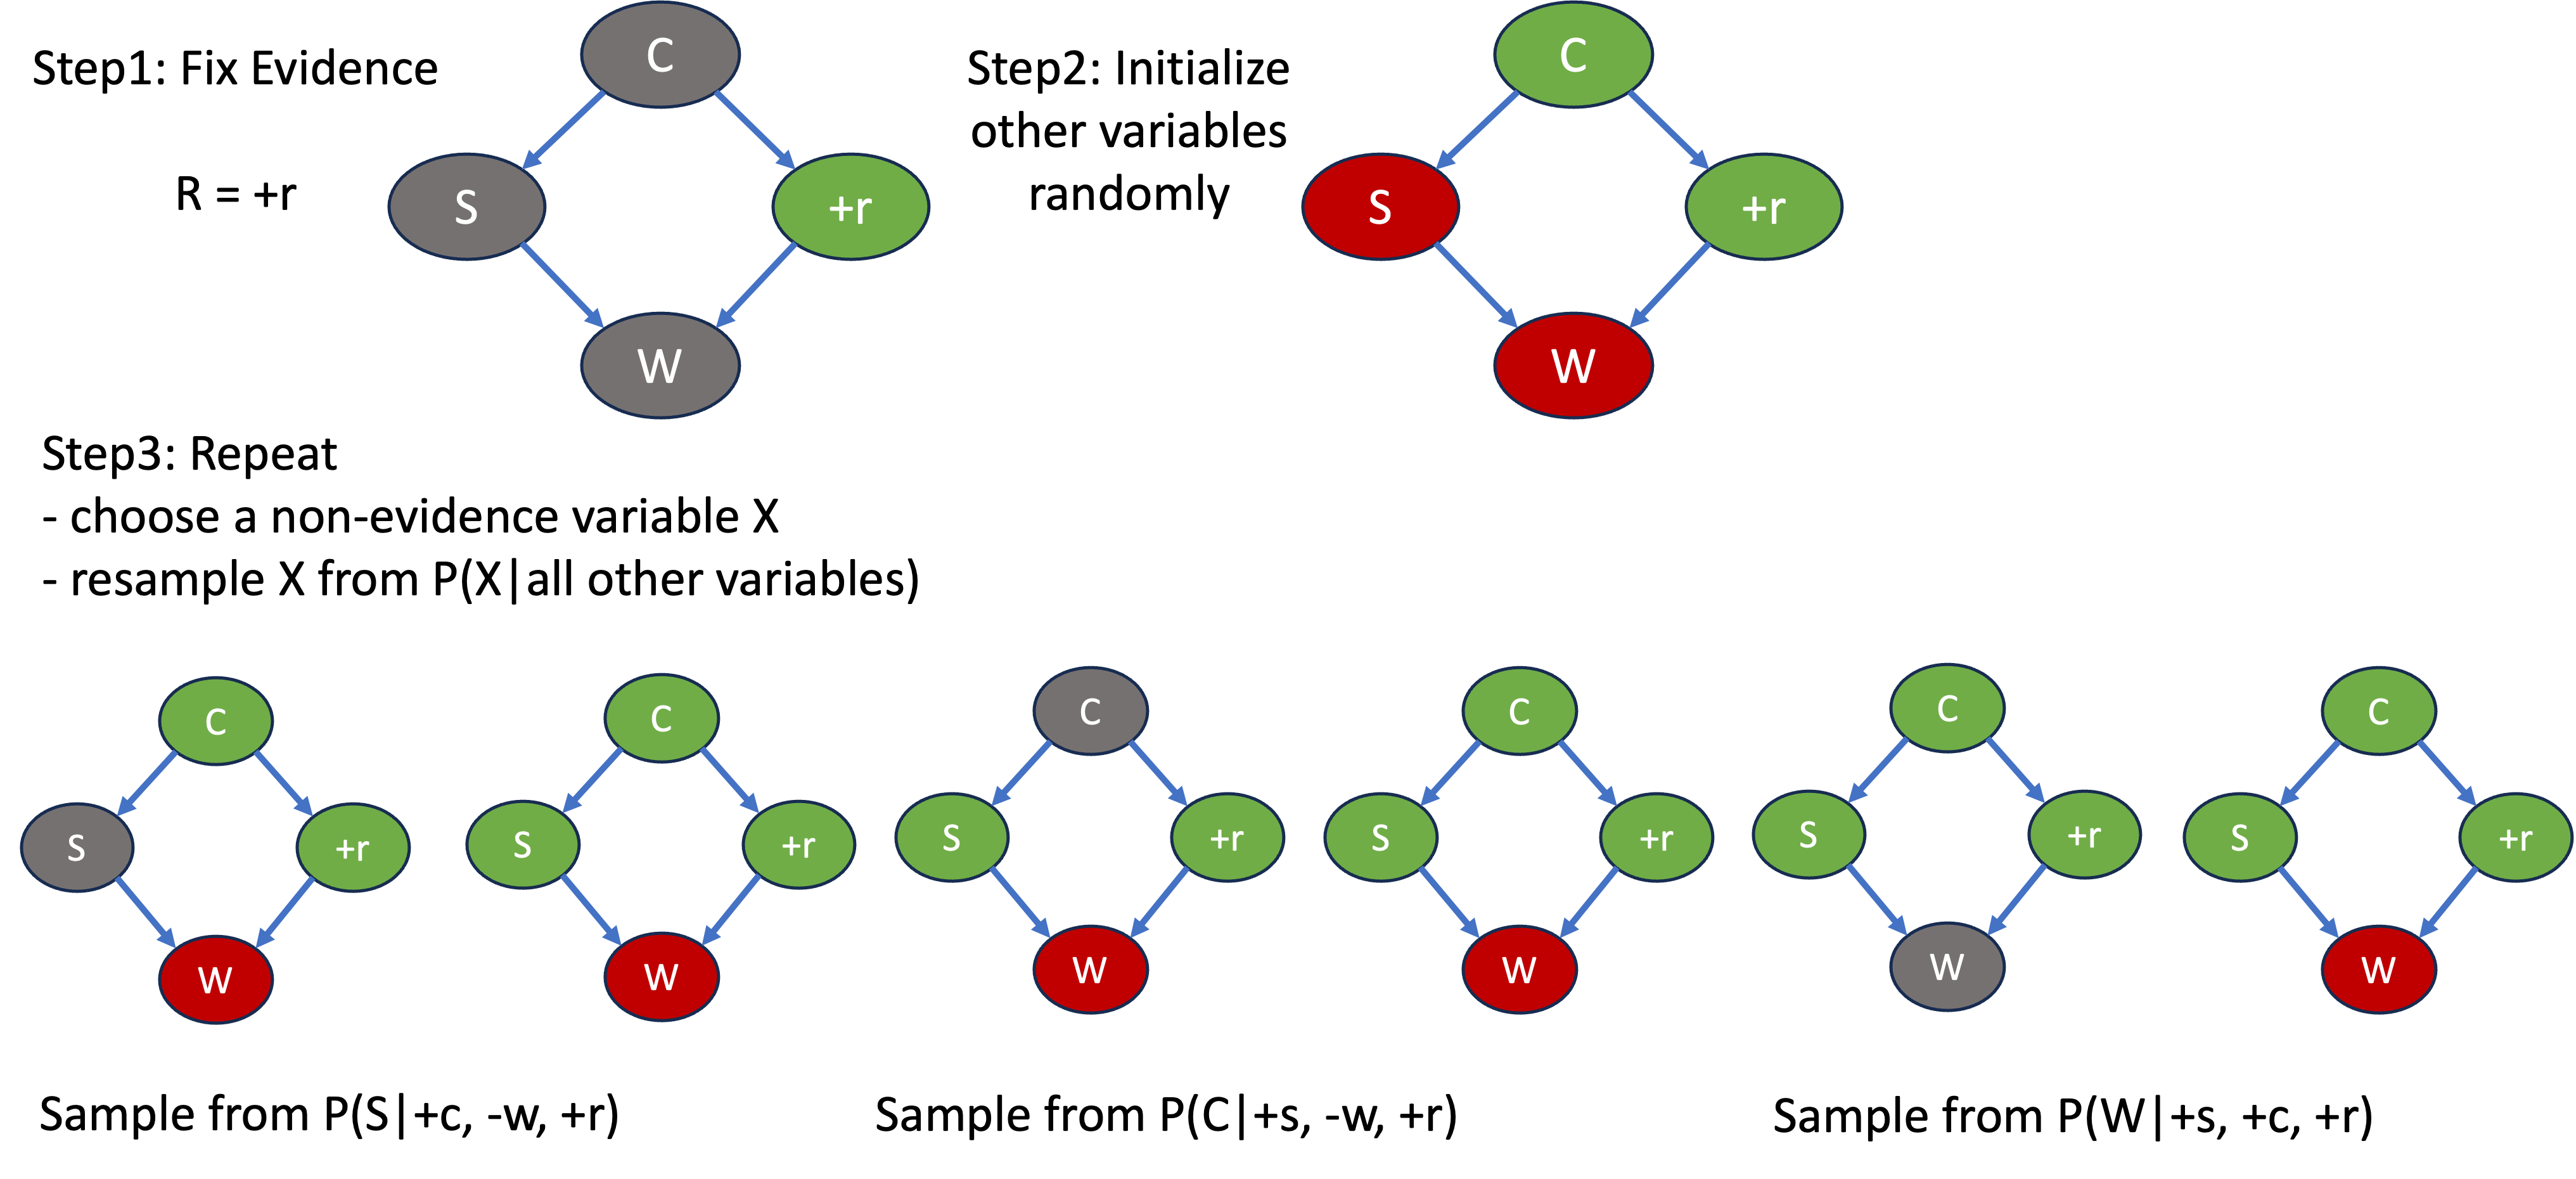
\includegraphics[width=15cm, height = 8cm]{gibbs.png}\\
\end{itemize}
















\end{document}
